% !TeX spellcheck = en_US 
\chapter{State of Research and Development}\label{chap2}
The following chapter gives a brief introduction to the topic of fatigue analysis in mechanical engineering. Further, the topic of ML with its core functionalities is presented. Finally, it is analyzed how ML is applied in industry, especially in fatigue analysis of machine elements.

\section{Introduction to Fatigue Life Analysis}
The goal of fatigue analysis is the dimensioning of machine elements in such a way that they are able to withstand the expected loads over an expected time period \cite{Haibach}. The strength of a machine element depends on the used material as well as the geometry \cite{Wittel}.

\subsection{Load Sequence and Load Spectrum}
The stresses resulting from repeated loading of a mechanical component can be plotted over time. This loading over time is referred to as load–time history. When omitting the time component and only keeping the order, it is referred to as the loading sequence \cite{HEULER}. In this thesis, the load–time history and loading sequence are treated as equal. In cases where the amplitude of the load in the loading sequence is not constant for each load cycle, the process is referred to as variable amplitude loading \cite{Facchinetti}.
Figure \ref{fig:VAL} shows a repeated loading with a constant and variable amplitude.
The resulting stresses are reaching a constant or varying level, depending on the load pattern. Depending on the area of application, the \(y\)-axes can also show a moment applied to a component like a driveshaft.

\begin{figure}[H]
	\centering
	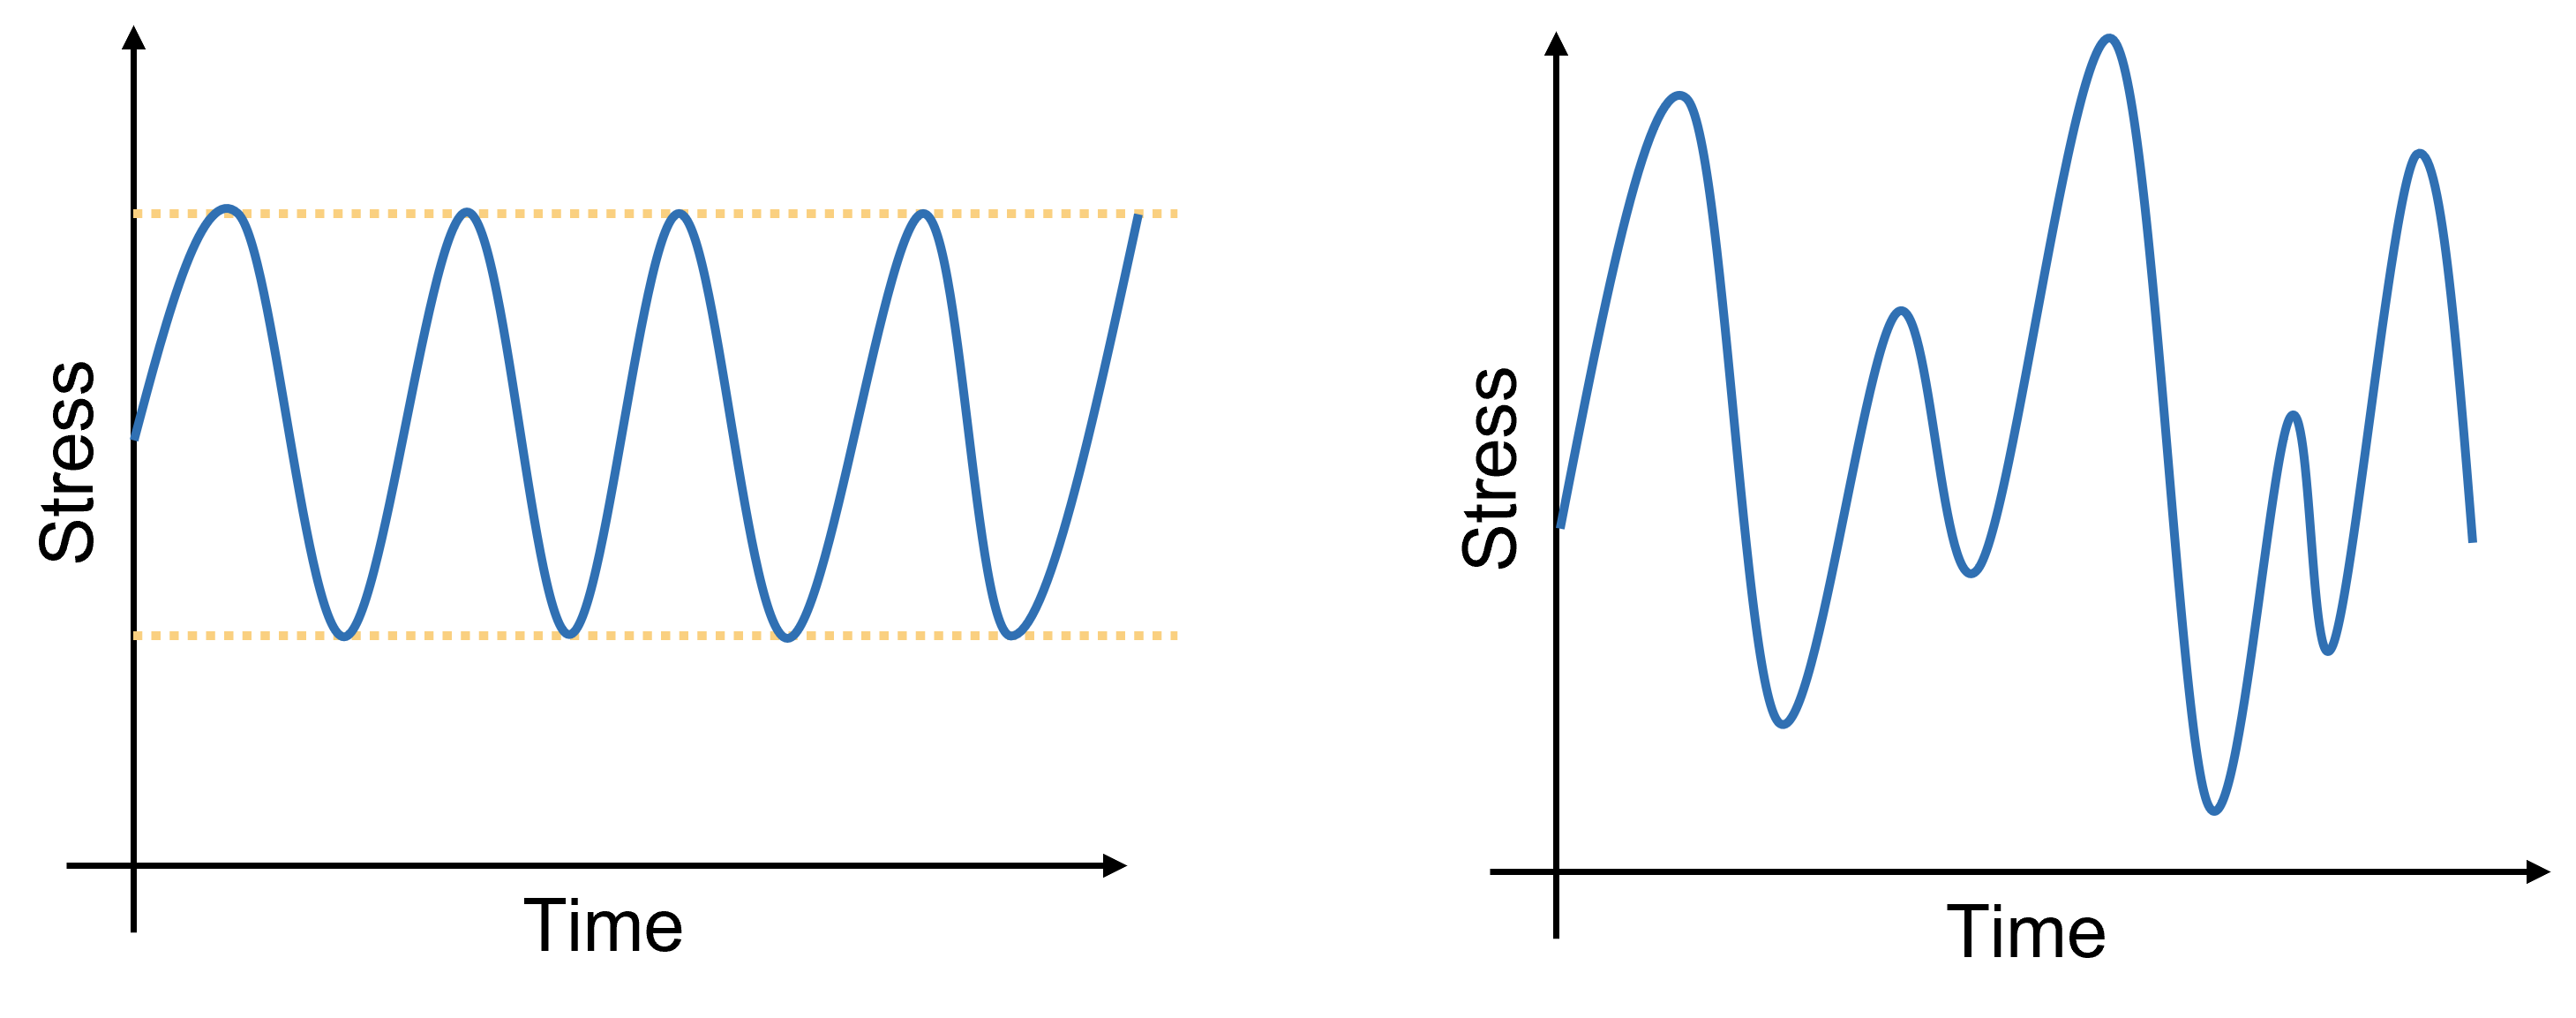
\includegraphics[width=0.8\linewidth]{IMGs/loading.png}
	\caption{Constant and variable amplitude loading}
	\label{fig:VAL}
\end{figure}
 
The Load Spectrum deals with the occurrence of load cycles with different amplitudes within a load sequence \cite{Facchinetti}. To get a load spectrum from a load sequence, the time and order component are omitted. A load spectrum shows the number of occurrences of a certain load amplitude in a load sequence.
By eliminating the order and time component of a sequence, the same load spectrum may arise from multiple different sequences. Depending on the desired detail in the load spectrum, the load levels of a sequence can also be rounded. Depending on the area of application, the rounding can be done to the next integer or the next 10,000.

The rounding will increase the occurrences at a certain load level as more occurrences are projected in each category. 
Figure \ref{fig:LS} shows a schematic load spectrum calculated from an exemplary load sequence.


\begin{figure}[H]
	\centering
	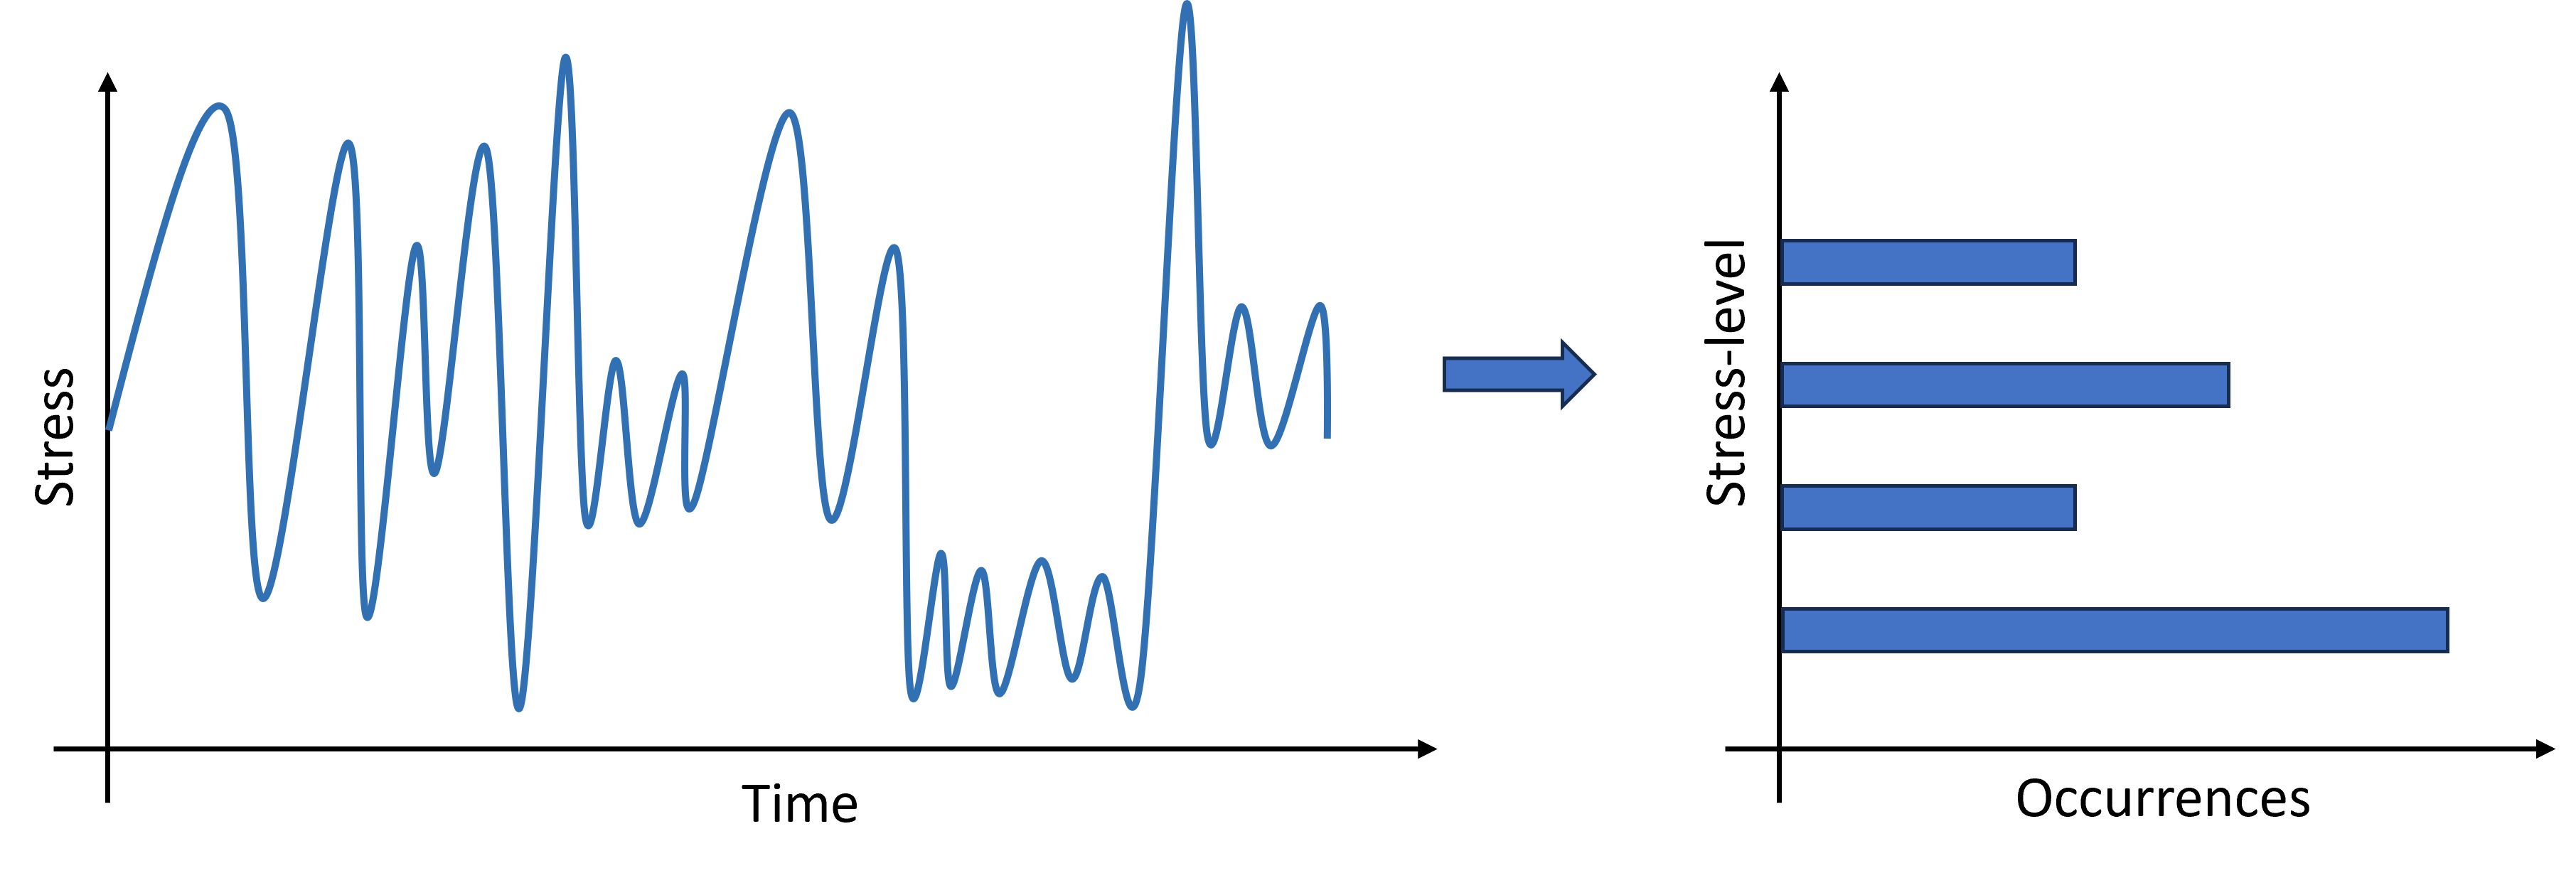
\includegraphics[width=0.95\linewidth]{IMGs/Spectrum.png}
	\caption{Load Spectrum from Load Sequence}
	\label{fig:LS}
\end{figure}

\subsection{The S-N Curve}\label{sn}
The S-N curve (also referred to as the Wöhler-curve) plays a very important role in fatigue analysis. It is applied in all aspects of engineering \cite{Burhan,Pungo}. 
The graphical representation gives clear insights into the maximum number of load cycles a material is capable of withstanding before a fatigue break is expected.
The applied load (S) is placed on the \(y\)-axes and the number of cycles (N) on the \(x\)-axes. The curve shows the number of cycles to fatigue failure and is individual for every material and for every different component.
The S-N curve can also be determined for elements like welded joints or whole structures \cite{Baptista, Dong}.
Both axes are on a logarithmic scale to achieve a straight line passing from the upper left to the lower right of the graph \cite{Little}.

Figure \ref{fig:WO} shows a schematic representation of the S-N curve: 

\begin{figure}[H]
	\centering
	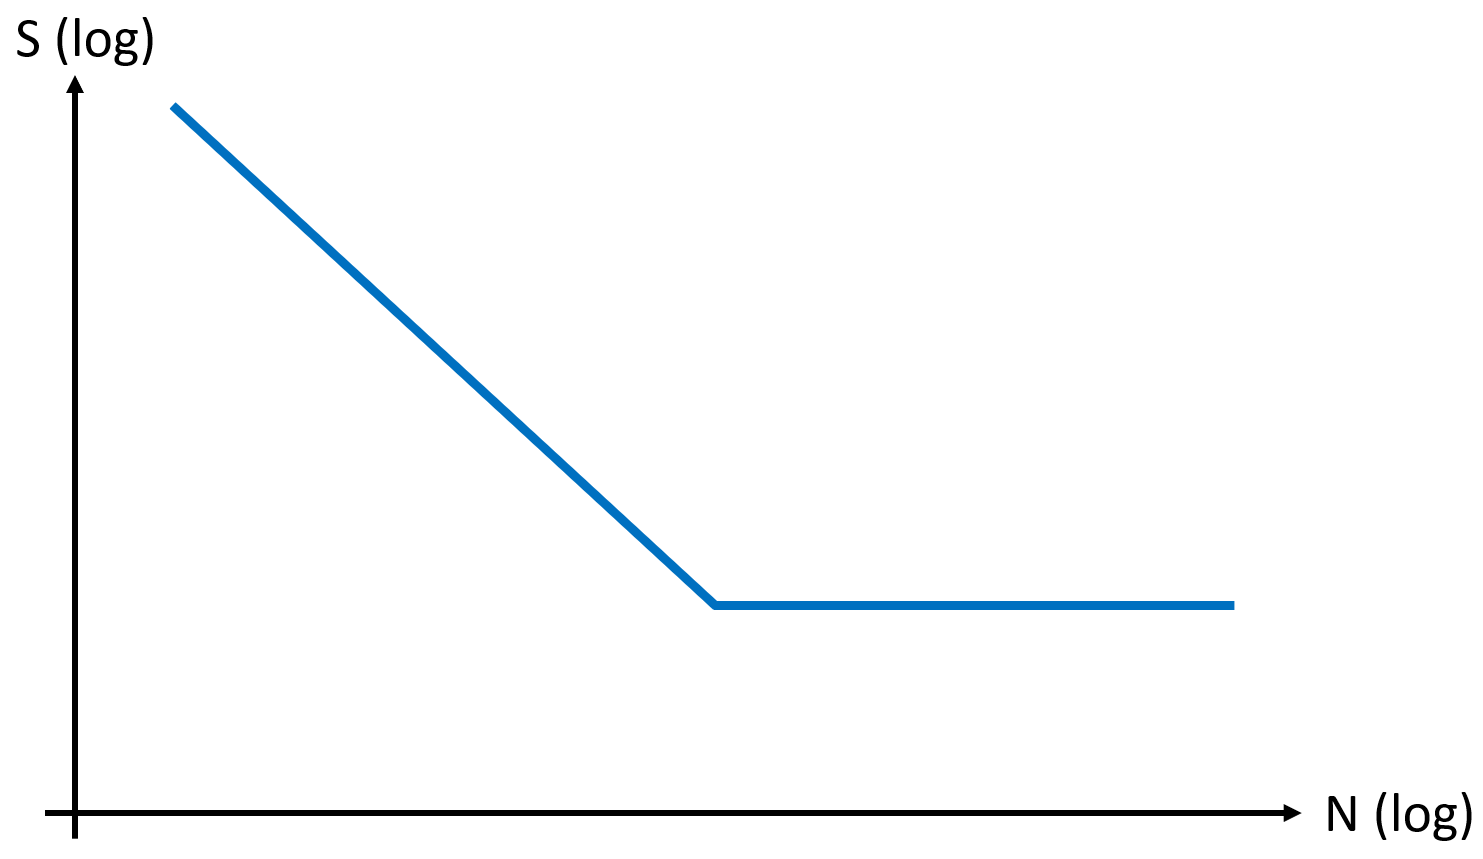
\includegraphics[width=0.7\linewidth]{IMGs/WO.png}
	\caption{Schematic representation of a S-N curve}
	\label{fig:WO}
\end{figure}
\newpage
As can be seen in figure \ref{fig:WO}, the curve is made up of two straight lines. The first part, which has a negative slope, is referred to as a fatigue strength range. In that range of loads, the material shows a limited number of cycles before failure occurs \cite{Adasooriya}.

The horizontal line marks the endurance limit, also known as the fatigue limit. Below that load level, it is assumed that a material can withstand an infinite number of cycles without failure \cite{Bellows}. It is often denoted as the S-N curve plateau.
It is important to note that the S-N curve is determined by experiments conducted in controlled environments and not on real-life machinery in industrial applications. Real-world applications may involve additional factors, such as varying load levels, environmental conditions, and surface finishes, which can influence fatigue performance \cite{JanOveHolmen}. 

Figure \ref{fig:WO2} gives a clear insight on how the S-N curve is actually a probability distribution and not a fixed deterministic line. This distribution arises from the different number of cycles achieved in experiments at the same stress level before failure occurred. Depending on the component and material, is not necessarily a Gaussian distribution. 

\begin{figure}[H]
	\centering
	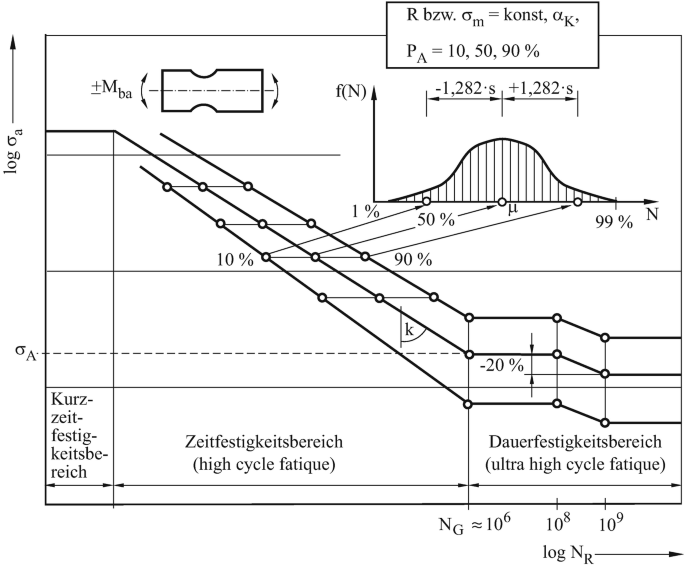
\includegraphics[width=0.7\linewidth]{IMGs/WO2.png}
	\caption{S-N as a distribution \cite{Klein}}
	\label{fig:WO2}
\end{figure}
\newpage
\subsection{Linear Damage Accumulation Method}\label{LAD}
The S-N curve is a crucial component in the application of the Miner rule \cite{MinerOG, Subramanyan}. The Miner rule is a popular linear damage accumulation technique most commonly used in engineering. It is based on three assumptions. First, that the rate of damage accumulation is constant over each loading cycle of one load level. Second, damage only occurs if the applied stress is higher than the fatigue limit (S-N curve plateau). This assumption is only true for the Miner-original and not for Miner-elementar or Miner-Haibach \cite{Werner}. And third, the component is expected to fail when cumulative damage reaches the unity \cite{Zuo}.
The Miner rule also assumes that the first load cycle at a certain stress-level is just as damaging as any other at that stress-level. The order of loads is not relevant when calculating the accumulated damage.

Each load-cycle damages the machine element inversely proportionate to the number of maximum loads the component could withstand at that stress-level. For example, if a component is capable of withstanding 1,000 loads at a certain stress level, one of those cycles adds 1/1000 to the accumulated damage of the machine element.
If another component can withstand 50 cycles at a different stress-level, each of those cycles adds 1/50 to the accumulated damage.

For varying loads, the sum of those individual ratios forms the accumulated damage. 
For example, 25 percent of the fatigue life is used up if a part is repeatedly loaded for 500 cycles at a stress level that would lead to failure in 4,000 cycles and then followed by 2,000 cycles at a stress level that would lead to failure in 16,000 cycles.
Equation \ref{acc} is how the accumulated damage-sum D is calculated. At stress-level \(S_1\), \(S_2\) ... \(S_i\), the corresponding numbers of load are \(n_1\), \(n_2\) ... \(n_i\). The number of cycles to failure under each stress level are \(N_1\), \(N_2\) ... \(N_i\).

\begin{equation}\label{acc}
	D = \sum_{j=1}^{k}\frac{n_i}{N_i}
\end{equation}

As mentioned before in chapter \ref{sn}, the individual points \(N_i\) in the fatigue strength range are determined by applying one load in a cyclic manner, to determine the maximum acceptable cycles. When using this number as a ground truth in the Miner rule, the effects of other loads, happening before or after, are neglected. To solve this, non-linear damage accumulation methods were developed.

\subsection{Non-Linear Damage Accumulation Methods}
One of the first non-linear fatigue damage accumulation models was the expansion of miner rule by a power law \cite{Zuo}.
Equation \ref{n1} shows how the damage sum D is calculated. The parameter \(C_i\) is a material parameter corresponding to the i-th loading level. 

\begin{equation}\label{n1}
	D = \sum_{j=1}^{k}\left [\frac{n_i}{N_i}\right ]^{{C_i}}
\end{equation}

The disadvantage of this method is that the parameter \(C_i\) must be calculated for different loading
conditions and thus tedious to acquire \cite{Zuo}.

Another approach, used in \cite{Rege}, proposes to use iso-damage-curves as a basis to calculate the cumulative fatigue damage.\newline
Many more approaches can be found in \cite{Zhu1,Gao,Lv,Chen}.

The common disadvantage of non-linear models is that they are dependent on very individual and specific parameters, limited to certain materials or loading histories, with a fixed trend regarding the loading amplitudes. Due to those limitations and cumbersome usage, they are not widely adopted in the engineering field \cite{Vietze}. 


\newpage
\section{Overview of Machine Learning}
In contrast to rigid algorithms, ML is a method that can solve a given problem without being explicitly told how to solve it \cite{Sutton,Janiesch}. The following chapter discusses the advantages, general functionality, and core principles of ML.

\subsection{General Introduction to Machine Learning}\label{General Introduction to Machine Learning}
ML is a subsection of the field of general AI \cite{Helm}. The same as deep learning (DL) is a subsection of ML \cite{LeCun}.
AI encompasses the general principles and methods that can mimic human behavior and decision-making \cite{Janiesch}. ML, on the other hand, incorporates all methods that can learn from data and discover regularity and patterns that are not obvious to a human~\cite{Theodoridis}. Based on the discovered knowledge, the trained model can be used to make predictions for new inputs in the future.
DL is a subset of ML that refers to methods that utilize a special approach called a Neural Network (NN). The "depth" in DL in this context refers to the amount of stacked layers of neurons (see chapter \ref{NN chapter}) \cite{Carleo}. 
DL is more capable than shallow ML and shows improved learning capabilities, but it also comes with its own specific challenges \cite{Janiesch, LeCun}.

Figure \ref{fig:AIMLDL} shows how DL and ML are subsets of AI. 

\begin{figure}[H]
	\centering
	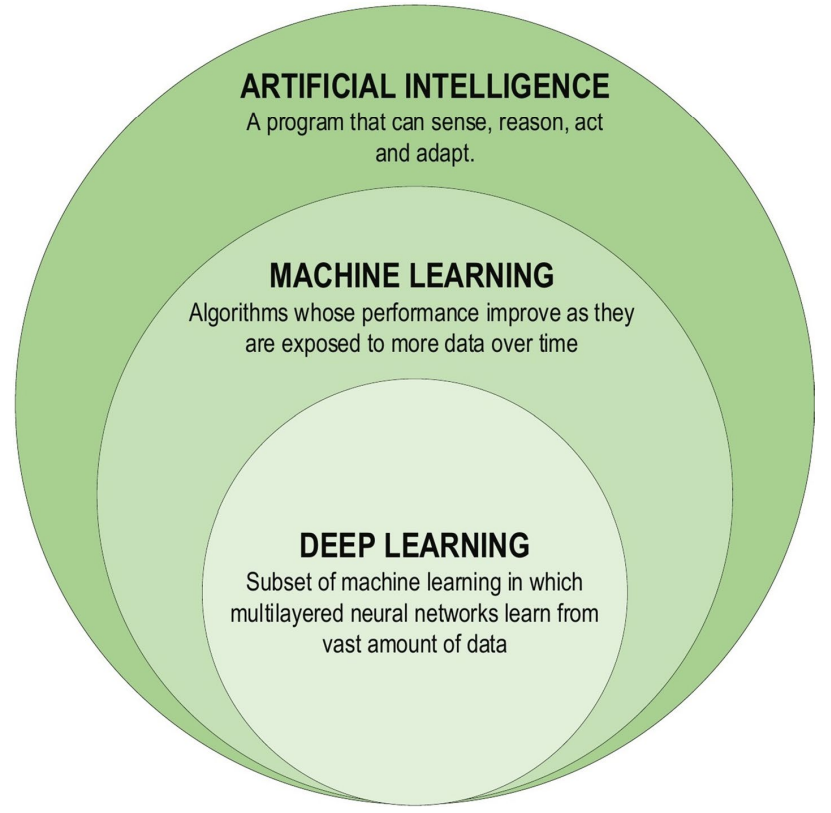
\includegraphics[width=0.7\linewidth]{IMGs/AIMLDL.png}
	\caption{Venn-Diagram of the different subsets of AI \cite{Alzubaidi}}
	\label{fig:AIMLDL}
\end{figure}
\newpage
\subsection{Advantages and Problems of Machine Learning}\label{Advantages and Problems of Machine Learning}
The most important \textbf{advantage} of ML is the ability to learn from data and discover the underlying, non-obvious patterns \cite{Wuest}. With that knowledge, it is also possible to predict the output for a specific input. A ML model deployed to a self-driving car could, for example, predict how a pedestrian is going to cross a street and calculate if the car should perform an emergency brake to avoid a collision. One further advantage of ML is its wide applicability \cite{Thommandru}. Not only computer science or the automotive industry, but also banking, healthcare, and many more fields, can all find applications where ML can help improve a process.

These algorithms are also very efficient and profit greatly from more available data \cite{Janiesch}. Not only is it possible to learn from a lot of data, but also to process a lot of data \cite{Wuest}. One example is the analysis of sensor data, for example, from LiDAR sensors. Those sensors produce a lot of data that might need to be analyzed as quickly as possible, in some cases even in real-time. For self-driving cars, fast analysis of this data is crucial for avoiding accidents. ML is capable of solving this problem reliably \cite{Lyu}. 

The era of "Big Data" plays right into the hands of ML. More data results in better performance of the ML approaches \cite{Wuest}. Also, the methods can be specially adapted to be robust. Outliers, noise, and missing values in the data do not skew the results in a significant way \cite{Theodoridis}. When comparing ML to DL, ML can tend to produce better results in cases where the training data is limited and also allows for a better interpretation of the outputs of the model \cite{Janiesch}.

The \textbf{disadvantages} of ML are closely related to the advantages. For example, the data-set that is used for training needs to be a certain minimum size so the model is able to learn the underlying patterns. But not only the size is important, but also the contained elements, as some models can return different results based on the elements that make up the data-set. The effectiveness of ML rises and falls with the amount and quality of the data \cite{Janiesch, Bishop}.

One of the biggest problems of ML is generalization \cite{Bishop}. Finding and learning patterns is just the first step, but making a correct prediction is the most valuable part. Depending on the free parameters of ML models, they have the capability to memorize the whole presented training-set and perform very poorly on data that is not part of the training-set \cite{Zhangpiml}. This case is called "over-fitting" \cite{Jabbar}. In such cases, the model does not learn the underlying structure of that data, but just the correct associations from one input to one output. 

The opposite of "over-fitting" is called "under-fitting" \cite{Jabbar}. The model is not capable of learning any patterns, and thus performs very badly on the training set and on newly presented test samples. This happens mostly when the data-set is not large enough for the chosen model or the model is not flexible enough to adapt to the pattern of the data \cite{Will}. In a worst-case scenario, a ML method could interpret the noise of the data as a pattern, and perform very poorly when applied in real-world applications.\newline

Especially for high-dimensional data and complex problems, a very large dateset is a must. This can be difficult to obtain, especially in the area of natural sciences or industry \cite{Wuest}. Sensors can provide very corrupt data, and some experiments can take a lot of time and money to perform. And if that data is acquired, it still requires a significant amount of manual work to bring it into a form where ML methods can work with it. To train a model, for example, to classify multiple bacteria cells, it first takes time to grow the bacteria, but then also to label all the pictures. For example, the MNIST data-set for number recognition contains 70,000 elements, that were all manually labeled \cite{Pavlo}. So depending on the area or application, it is impossible to obtain a data-set that has the necessary size and quality. 

Further, models can be very susceptible to hyperparameters \cite{Janiesch}. Hyperparameters are fixed values that describe the characteristics of a model. Those values are set manually and require extensive knowledge about the implemented model, the problem at hand, and the available data-set \cite{Luo}. The optimal parameters can be found with an extensive brute force approach or specialized algorithms, but they require too much time to be feasible in an industry-application~\cite{Claesen}. 

Table \ref{AdDis} summarizes the advantages and disadvantages of ML. Despite its disadvantages, the abilities and unique advantages of ML make it a very interesting addition to industry applications~\cite{Bertolini}. Especially as more and more capable methods are developed. The main goal when implementing ML is to work around the disadvantages to achieve the desired results.


\begin{table}
	\begin{center}
	\begin{tabular}{|| c | c ||}
		\hline
		\rule{0pt}{2ex}
		 Advantages of ML & Disadvantages of ML \\
		\hline
				\rule{0pt}{2ex} 
		$\bullet$ can learn from data & $\bullet$ requires large datasets \\
		$\bullet$ can make predictions based on learned patterns & $\bullet$ data is tedious to acquire\\	
		$\bullet$ versatile in applicability & $\bullet$ is sensitive to hyperparameters\\
		$\bullet$ can process a lot of data efficiently & $\bullet$ can be sensitive to training-set\\
		$\bullet$ can handle noise and outliers in data & $\bullet$ over-fitting / under-fitting\\
		\hline
	\end{tabular}
	\caption{Advantages and Disadvantages of ML}
	\label{AdDis}
\end{center}
\vspace{-4mm}
\end{table}
\newpage
\subsection{General Terms in Machine Learning}
In the following, some of the general terms in ML are explained. As the field of ML is very large and continuously growing, this section focuses only on the core elements. Understanding these terms and principles helps to get a better understanding of the ML methods and how they can be applied in industry. For a more in-depth look, more information can be found in extensive literature \cite{Theodoridis, Bishop, google}.

\subsubsection*{Training and Testing}\label{TT}
To train and test the model's ability to generalize, the data is split up into a training-set and a test-set. The training-set is used to determine the optimal parameters of the model \cite{Bishop}. The process of finding the optimal parameters is referred to as training or learning. It is important to keep both sets separate and only use them for their respective purposes. The training-set must not contain elements of the test-set and vice versa. Otherwise, if the expected error is computed on the training-set, the ability of the model to generalize is not correctly assessed \cite{Xiaogang}.

One easy way to understand the search for optimal parameters during training is with the example of curve-fitting of a polynomial function (see \cite{Bishop} for a more in-depth look). \newline
Function \ref{fun1} is a polynomial of degree \(M\) with free parameters \(w_i\) that can be adapted to fit the data as accurately as possible.
The error function, defined in equation \ref{err1}, also called loss function, measures the accuracy of the polynomial. The parameters are changed in such a way to reduce the error. If the polynomial is flexible enough, the error is reduced to zero. In the case of ten free parameters and ten data points (\(x_n\),\(t_n\)) the polynomial passes through every data point exactly. The error in that case is zero. 
\begin{equation}\label{fun1}
	y(x,w) = \sum_{j=0}^{M}w_ij^j= w_0+w_1*x^1+w_2*x^2+...+w_M*x^M
\end{equation}
\begin{equation}\label{err1}
	E(w) = \frac{1}{2}\sum_{n=0}^{N}\{y(x_n,w)-t_n\}^2
\end{equation}

Figure \ref{fig:poly} shows how the polynomial changes based on the number of free parameters. When the polynomial, displayed in red, reaches degree nine, the error is zero. In this case, however, it is not following the true data generation function shown in green and performs very poorly on new unseen data points (see "over-fitting" in chapter \ref{Advantages and Problems of Machine Learning}).
%from \cite{Bishop}
\begin{figure}[H]
	\centering
	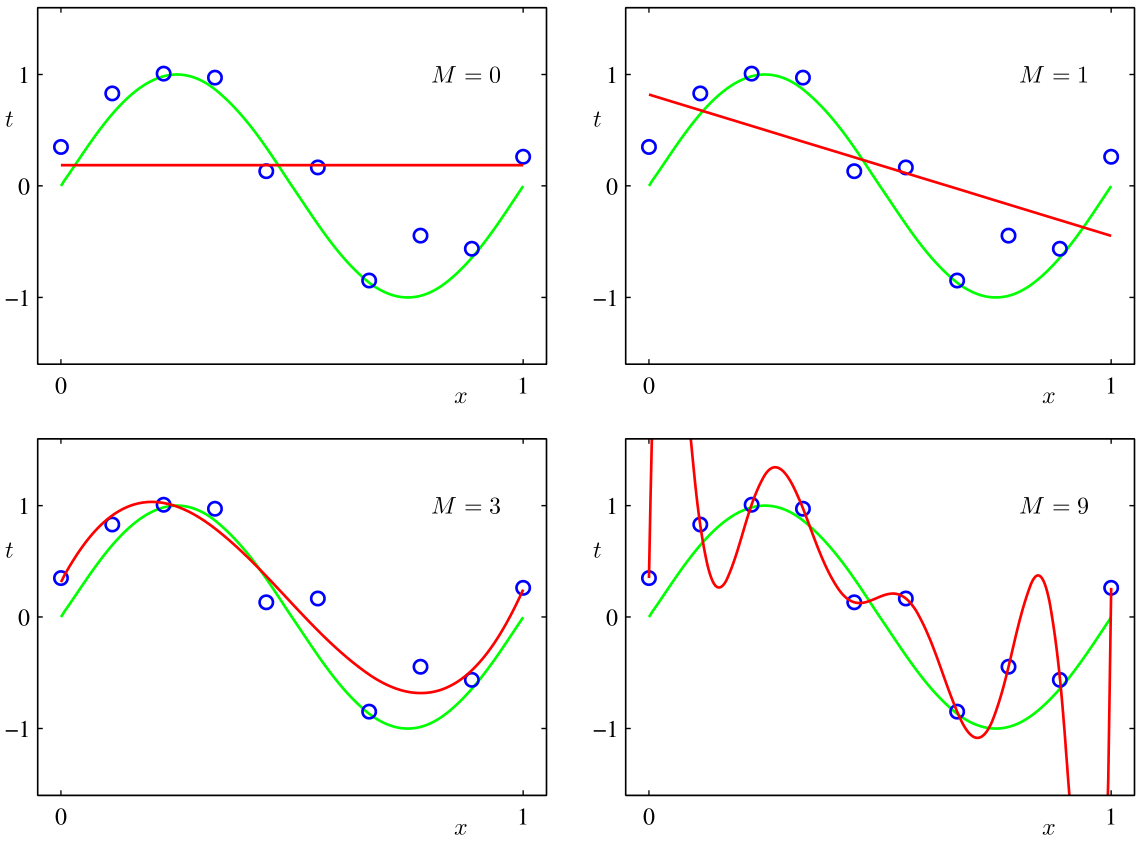
\includegraphics[width=0.8\linewidth]{IMGs/poly.png}
	\caption{Influence of the number of free parameters in curve-fitting \cite{Bishop}}
	\label{fig:poly}
\end{figure}

\subsubsection*{Features and Feature Selection}
Every model needs an input and a corresponding output. As computers work on a digital principle, physical values have to be transformed into a digital format. For example, sensor data from analog pressure valves or analog current meters has to be transformed into digital values.\newline "Industrie 4.0" did a lot of work to replace standalone analog sensors with sensors having a digital output or wireless connection, so that this translation step is no longer a hurdle. The post-processing of those signals can be done on a central computer or dedicated edge devices on the shop floor \cite{Lu}.

But not all data is accepted by a ML model right away, even if it is in digital form. These methods need an input that is specifically shaped for each specific model.
When the goal is to apply a ML model for image classification, the image needs to be transformed into a format that is accepted by the implemented model. Images can have different height-to-width ratios (e.g.,~16:9 or 4:3) and different resolutions (e.g.,~1920x1080 pixel or 64x64 pixel). All the images need to be transformed into a uniform shape with the same resolution \cite{Park}.

For example, if an image data-set contains mostly images with a 1:1 ratio, wider images need to be contracted or cut off to fit the pattern so that all images are the same. The resolution must also be adjusted so that all images have the same number of pixels.
\newpage
Figure \ref{fig:pixel} shows how images of different sizes and resolutions are adapted to a fixed resolution and ratio. In the upper image, the overhanging parts on the sides are removed, and no resolution scaling is necessary. In the lower image, parts on the top and bottom are removed. Additionally, the resolution was downscaled from 125x125 pixel to 100x100 pixel. 

\begin{figure}[H]
	\centering
	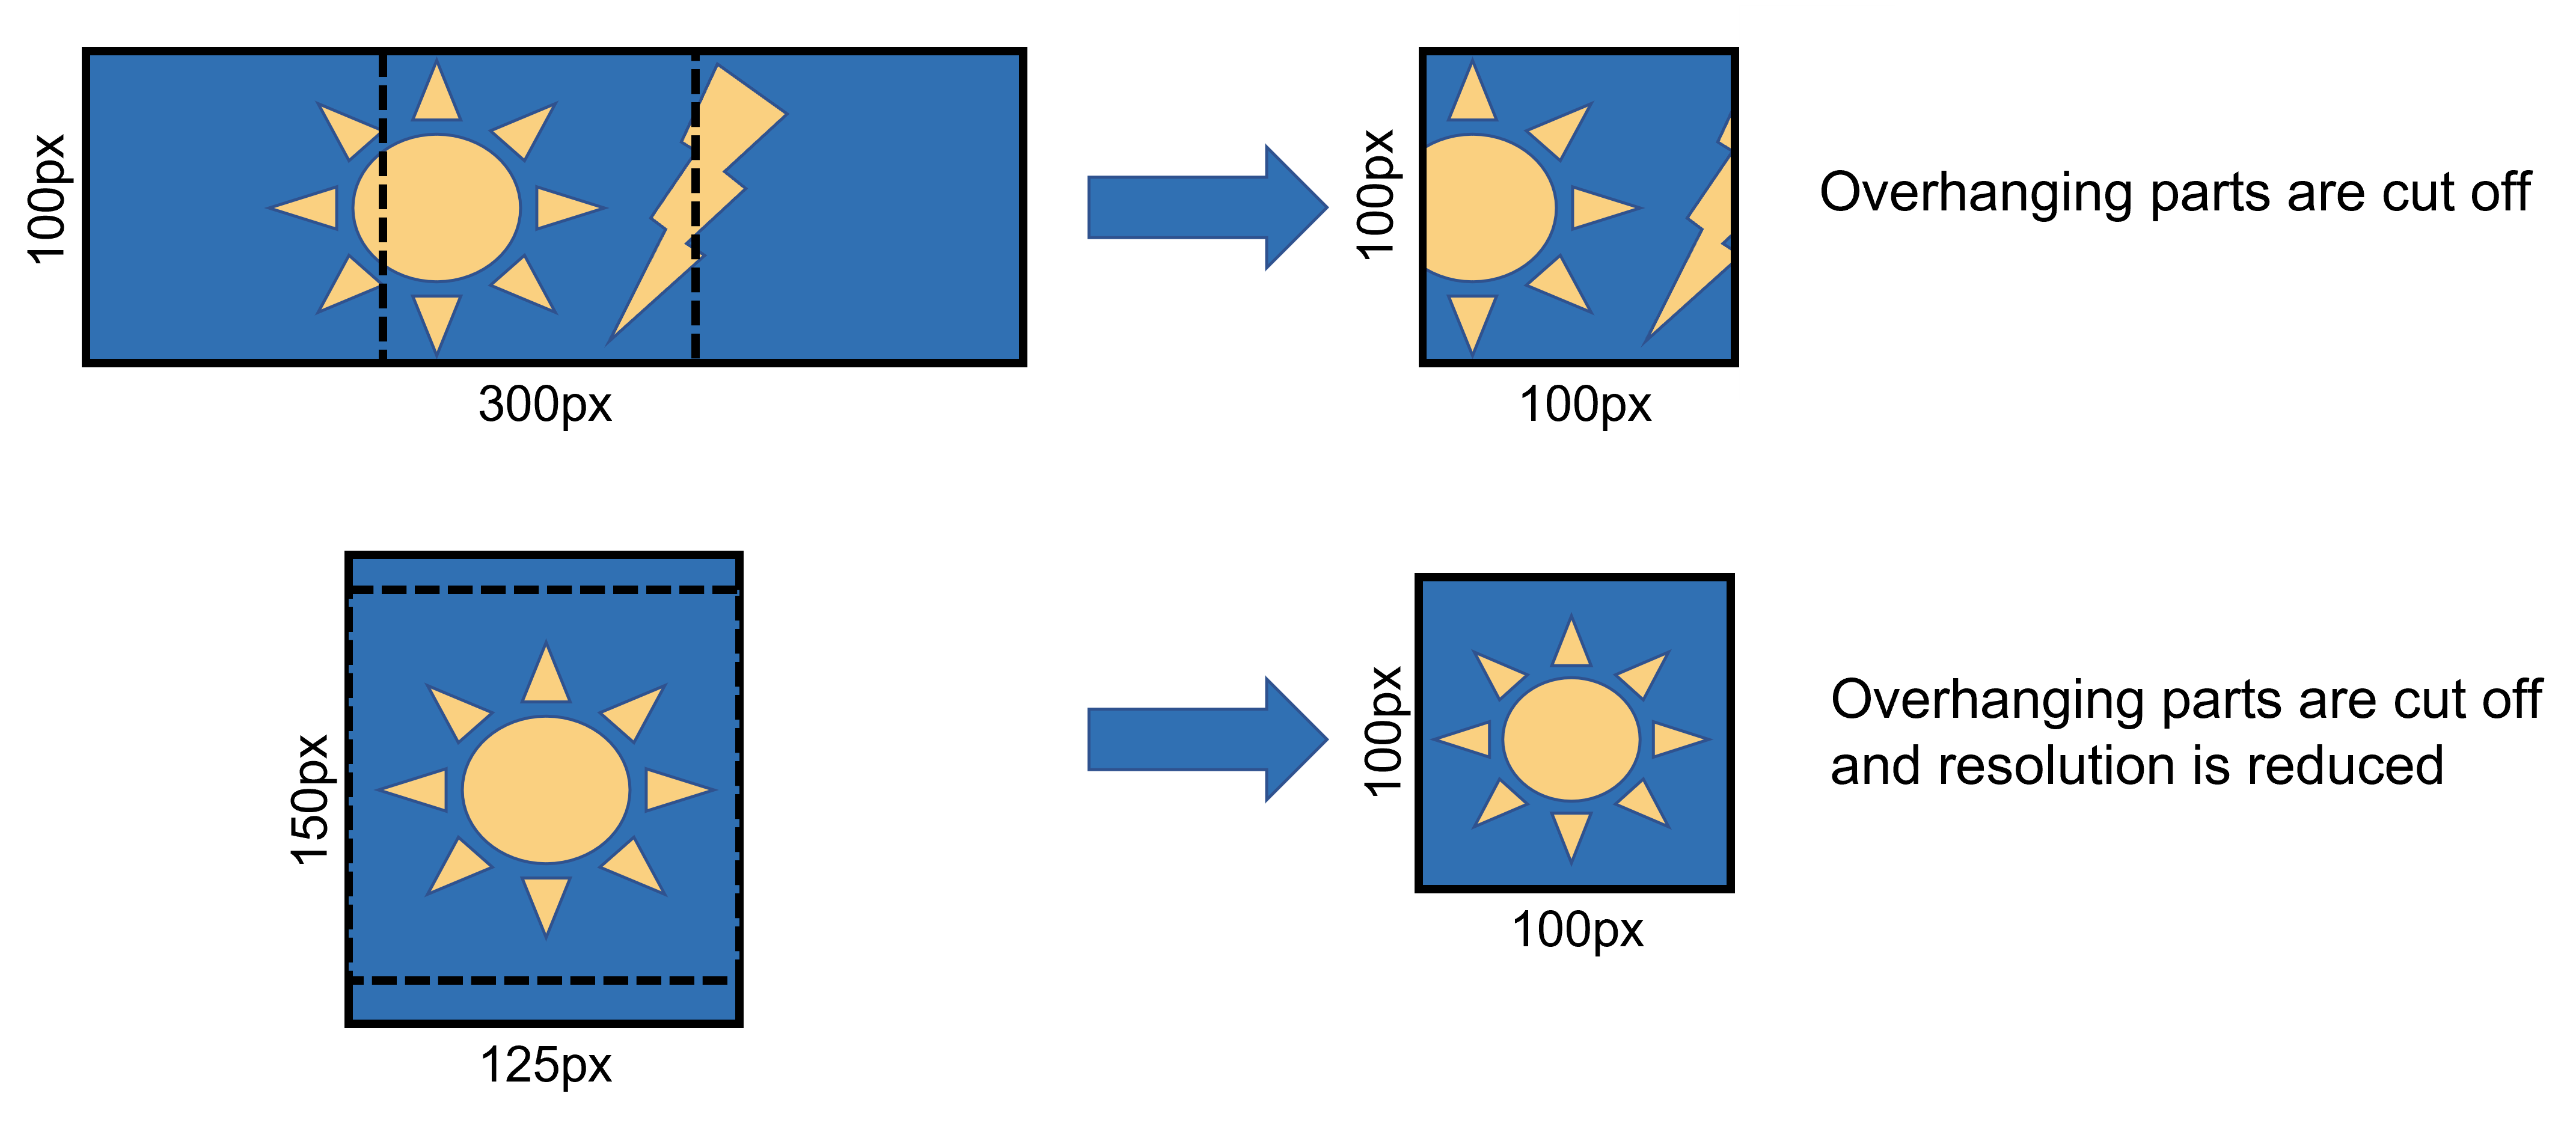
\includegraphics[width=0.95\linewidth]{IMGs/pixel.png}
	\caption{Changing resolution and ratio of images for a homogeneous data-set}
	\label{fig:pixel}
\end{figure}

The ratio and resolution depend on the implemented method and can be chosen freely. 
The current standard for images (MNIST) that are used in bench-marking of various algorithms is a squared format with a 28x28 pixel resolution \cite{Baldominos}.\newline
For optimal classification, a higher resolution proves advantageous but can require longer training times and more complex~models~\cite{Kannojia,Huang}.

After the input elements are standardized, they can be transformed into a vector or matrix format. The process of constructing such designed input from raw input is called "encoding". The result after the encoding is called a "feature vector". The elements of such a vector are referred to as features. One set of features uniquely represents the uncompressed input \cite{Theodoridis}. It is possible to reduce the feature vector through a process called "feature selection", where the feature vector is reduced even further to a smaller size that contains the gist of the raw input. By reducing the dimension, the models are capable of learning faster, but this process is running the risk of omitting valuable data in the process \cite{Janiesch}.

Figure \ref{fig:encoding} shows how a matrix, representing an image, for example, can be encoded as a vector. As long as the encoding method is constant for all input elements, the order is irrelevant. In that case, the elements can also be stacked not only row-by-row but also column-by-column.

\begin{figure}[H]
	\centering
	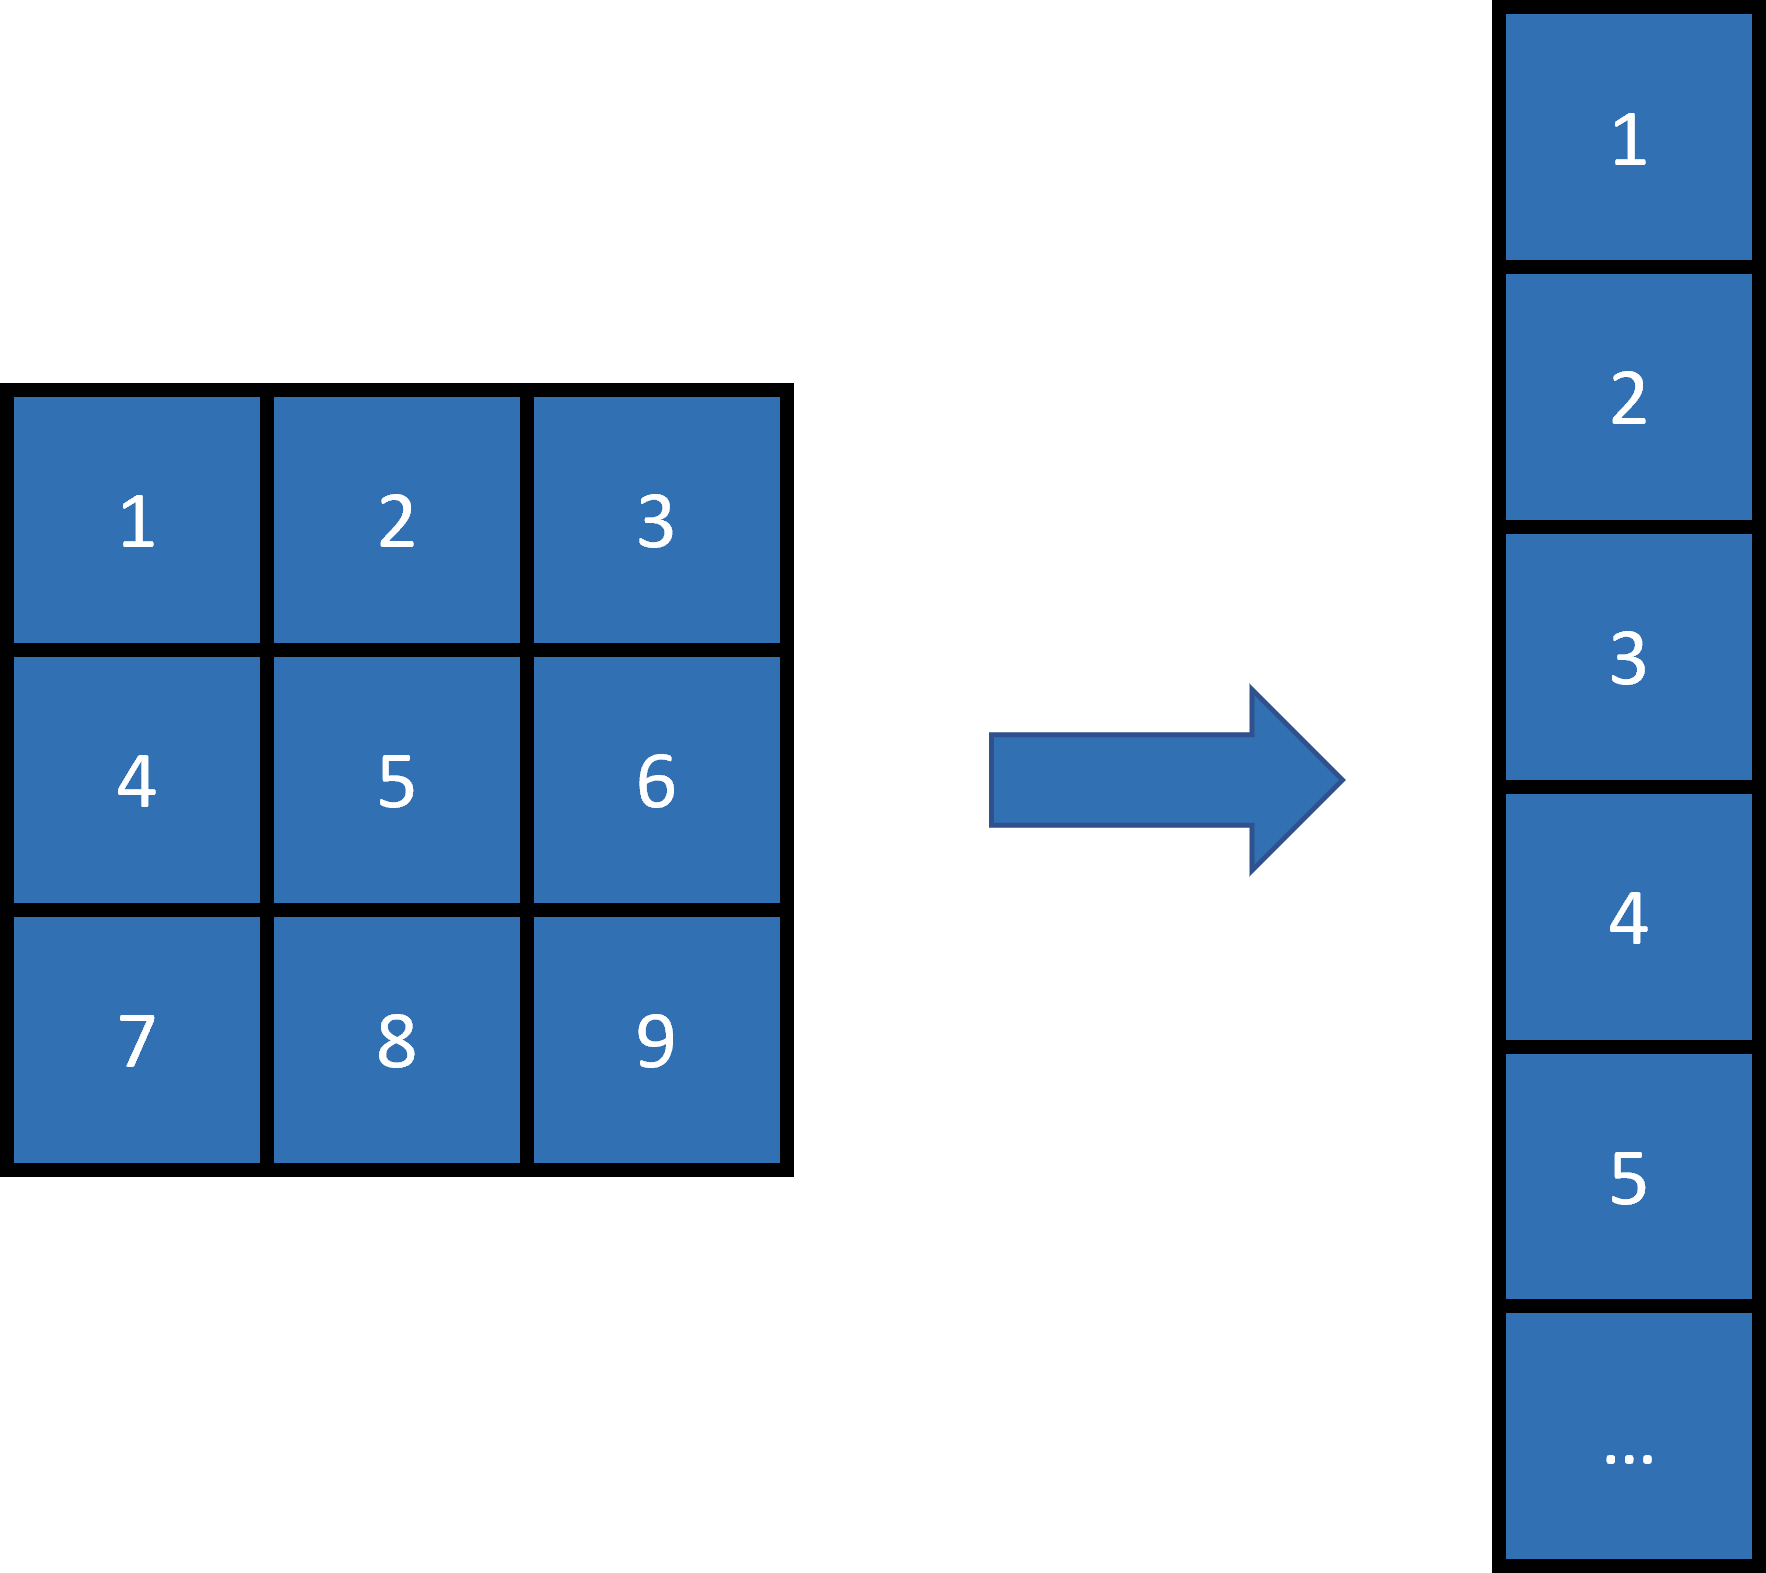
\includegraphics[width=0.455\linewidth]{IMGs/encoding.png}
	\caption{Encoding of an image-matrix as a vector}
	\label{fig:encoding}
\end{figure}

 
\subsubsection*{Data augmentation}\label{DAUG}
As mentioned in chapter \ref{Advantages and Problems of Machine Learning}, a large data-set improves the success of ML approaches. Instead of inflating a data-sets with noisy or corrupt samples and relying on the algorithm's ability to handle such data, a different approach is possible. The process of enlarging a given data-set is called Data Augmentation (DA). The goal is to bypass the problem of small datasets and increase their size and quality \cite{Shorten}. By doing so, over-fitting can be prevented. DA is mostly used on images, but can also be transferred to all other types of data. Possible DA approaches are, for example, geometric transformations like cropping, flipping, scaling, and rotating \cite{Taylor}. Further possibilities are changing the contrast, brightness, white-balance, tint of the image, as well as local pixel manipulations \cite{Mikolajczyk}. These individual adjustments can also be combined to produce a plethora of data.

Further approaches are possible when working with data in a time-series format \cite{Bandara, Wen}. One definition of time-series, is data that has a time component, like recorded sensor data, and thus can be plotted over time \cite{Hamilton}. Another definition is that the data has an orderly element and not necessarily a time component \cite{Iwana}. An example of a series without a time component are words in sentences. In such cases, cropping might distort the data too much to be representative of the original element.

One of the most straightforward approaches when working with signal data is to overlay the data with Gaussian noise or any other noise pattern. Another option is inserting or emitting repeating values of the data, which makes the time-series longer or shorter \cite{Wen}.

Figure \ref{fig:DA} shows further possible DA techniques. The different methods can be divided into basic and advanced approaches \cite{Wen}.

\begin{figure}[H]
	\centering
	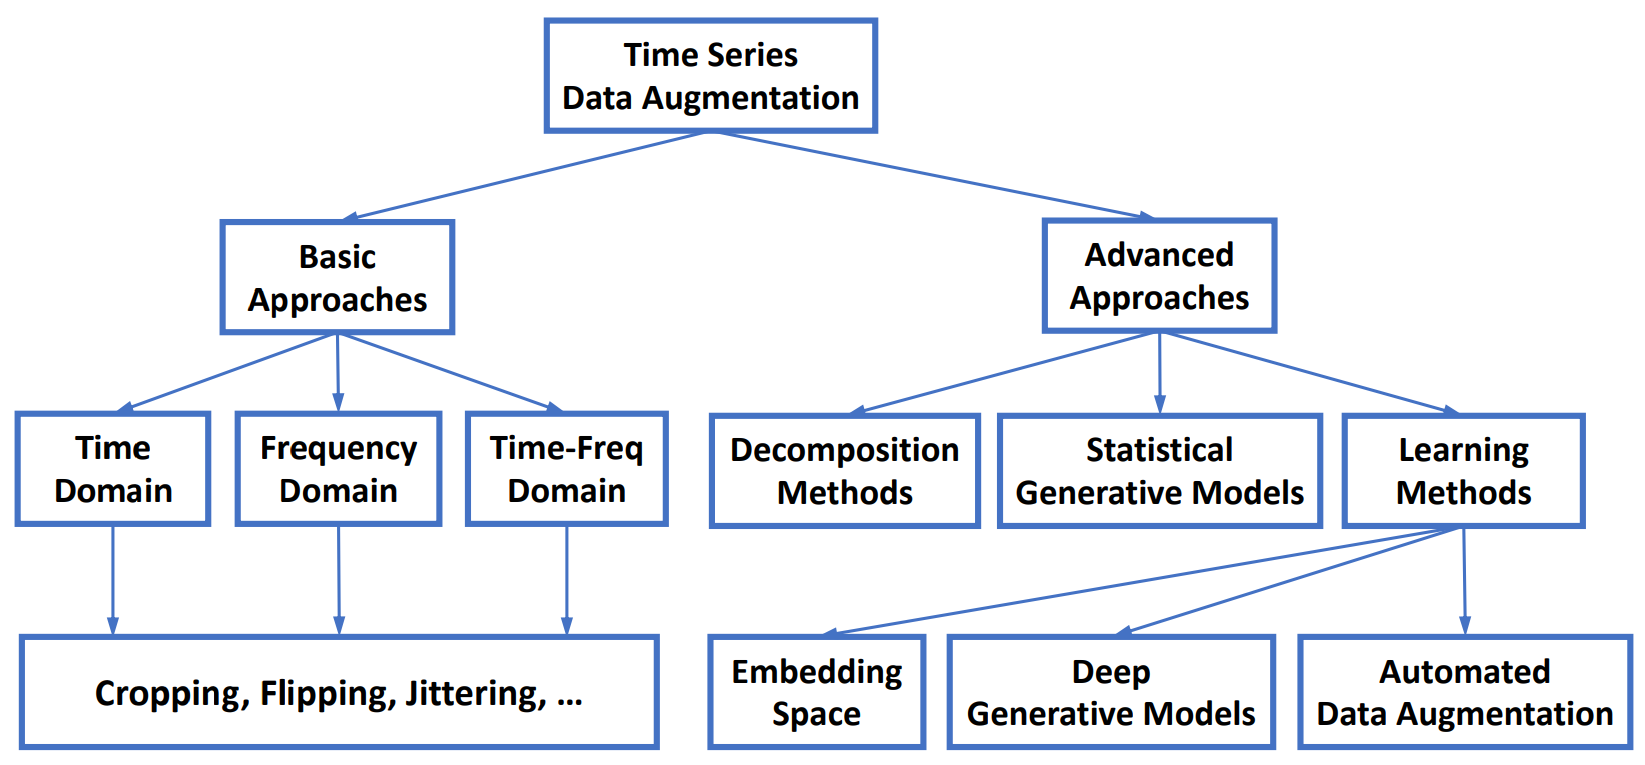
\includegraphics[width=0.9\linewidth]{IMGs/DA.png}
	\caption{Possible DA techniques for time-series data \cite{Wen}}
	\label{fig:DA}
\end{figure}

Figure \ref{fig:DA2} shows how a polynomial can be varied to increase the data-set size but still keep its significant characteristics.

\begin{figure}[H]
	\centering
	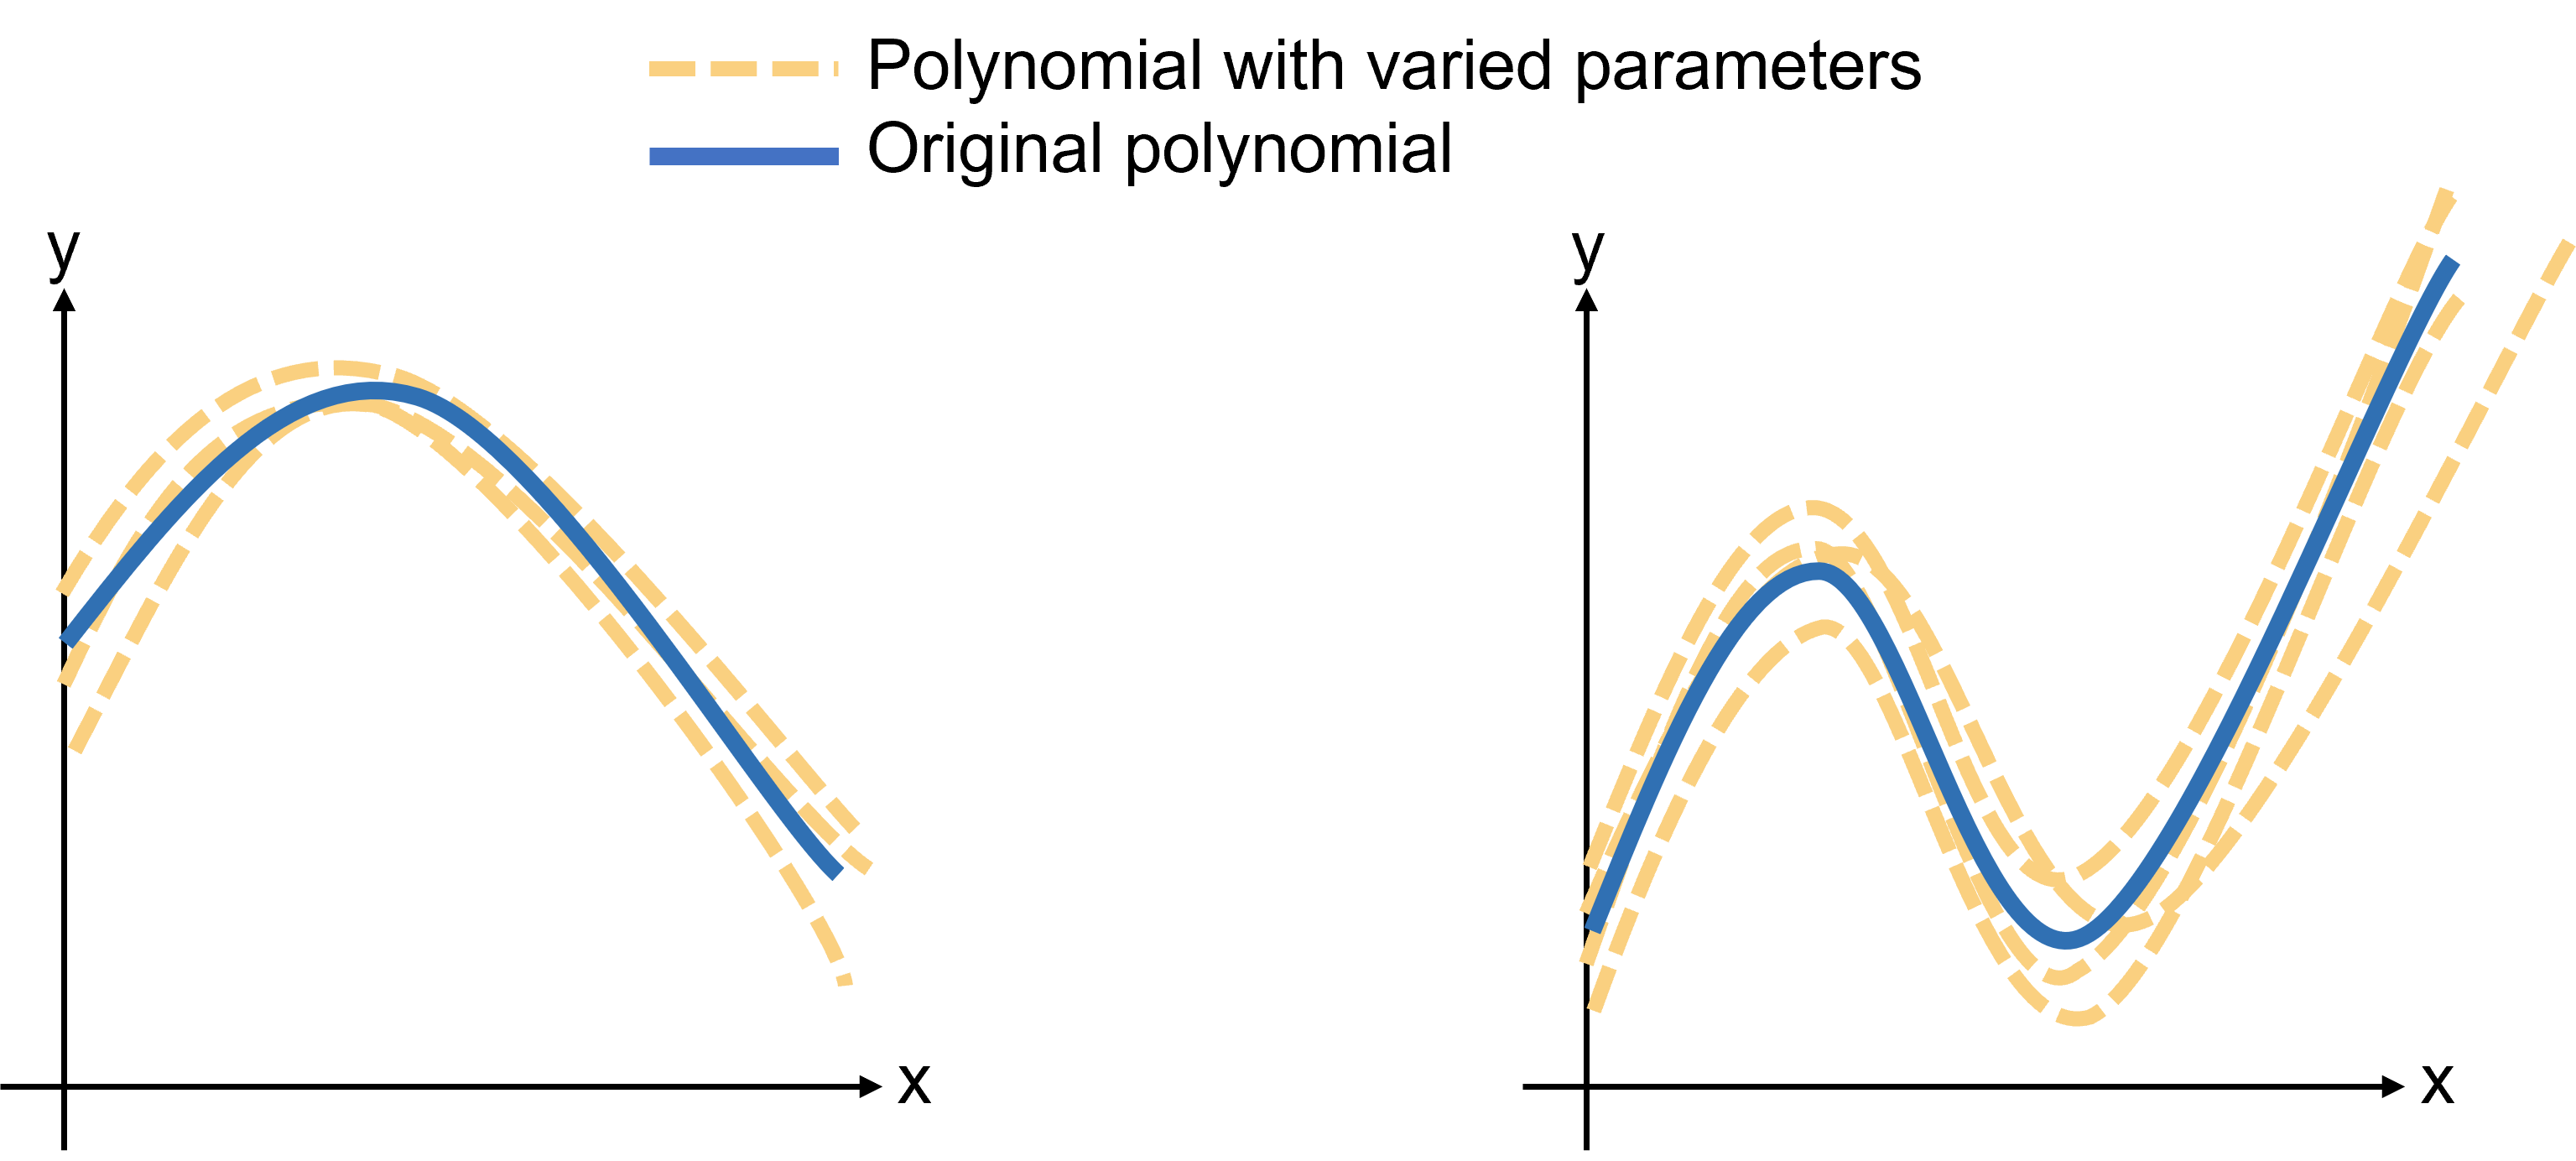
\includegraphics[width=0.8\linewidth]{IMGs/DA2.png}
	\caption{Application of DA to polynomial functions}
	\label{fig:DA2}
\end{figure}

\subsubsection*{Data Pre-Processing}
When working with a given data-set, it is helpful to the ML method if all feature vectors are in the same range across all samples.
The aim is that the greater numeric feature values are not dominating the smaller numeric feature values and each one can have an equal contribution to the output. This improves the performance of ML-methods significantly \cite{Singh}. The process of changing the data is referred to as pre-processing. In the following, a few selected data pre-processing methods are discussed in detail.

The first, and one of the most important pre-processing steps is the removal of outliers \cite{Yang}. Outliers can be values that do not fit the range of expected values or have no entries (missing data). In some circumstances, these data points are easy to filter out, as they can be compared to the real-world processes where that data was recorded. For example, a temperature recording from a melting furnace is expected to be in the range of 600 to 1000 degrees Celsius. Negative and close-to-zero values can be easily removed, as these values are not physically possible during operation. Removing outliers reduces the variance of the training set and is responsible for a significant performance boost \cite{Li}.

Normalization (also called Min-Max scaling or Min-Max Normalization,) is the process of projecting the data into a specific interval. This interval is most commonly set between~-1~and~1~\cite{Peshawa}. This method of scaling produces good results only if no outliers are present in the data-set. The outliers could skew the scaling such that the non-outlier values are projected onto a very small range of the interval and are very difficult to be distinguished from one another. The task of normalization is frequent in feature engineering. When all the numerical features in the feature vector fall within approximately the same range, models often train more quickly (and make better predictions) \cite{Jayalakshmi}.

The standardization approach involves remapping the features by subtracting the mean and dividing by the variance. This approach is used if the data is made up of multiple sources and the elements are not on the same scale. The data is standardized to prevent characteristics with wide ranges from impacting the output compared to the other values. Data is standardized to make it center on a certain value (0 is chosen most often) with a variance of 1 \cite{Raju}.
One example of standardization is when a future vector contains the pay and the years of employment of an employee. As the pay is numerically much larger than the years of employment, it is necessary to standardize all the elements across all feature vectors. 

Further possible pre-processing options include MaxAbs-scaling, Robust Scaler-scaling, and Quantile Transformer \cite{Ahsan}.
Figure \ref{fig:MM} shows how elements of a feature vector are projected in the range [-1;1] with the help of a MinMax-scaler. After the projection, numbers four and five are no longer distinguishable. 
\begin{figure}[H]
	\centering
	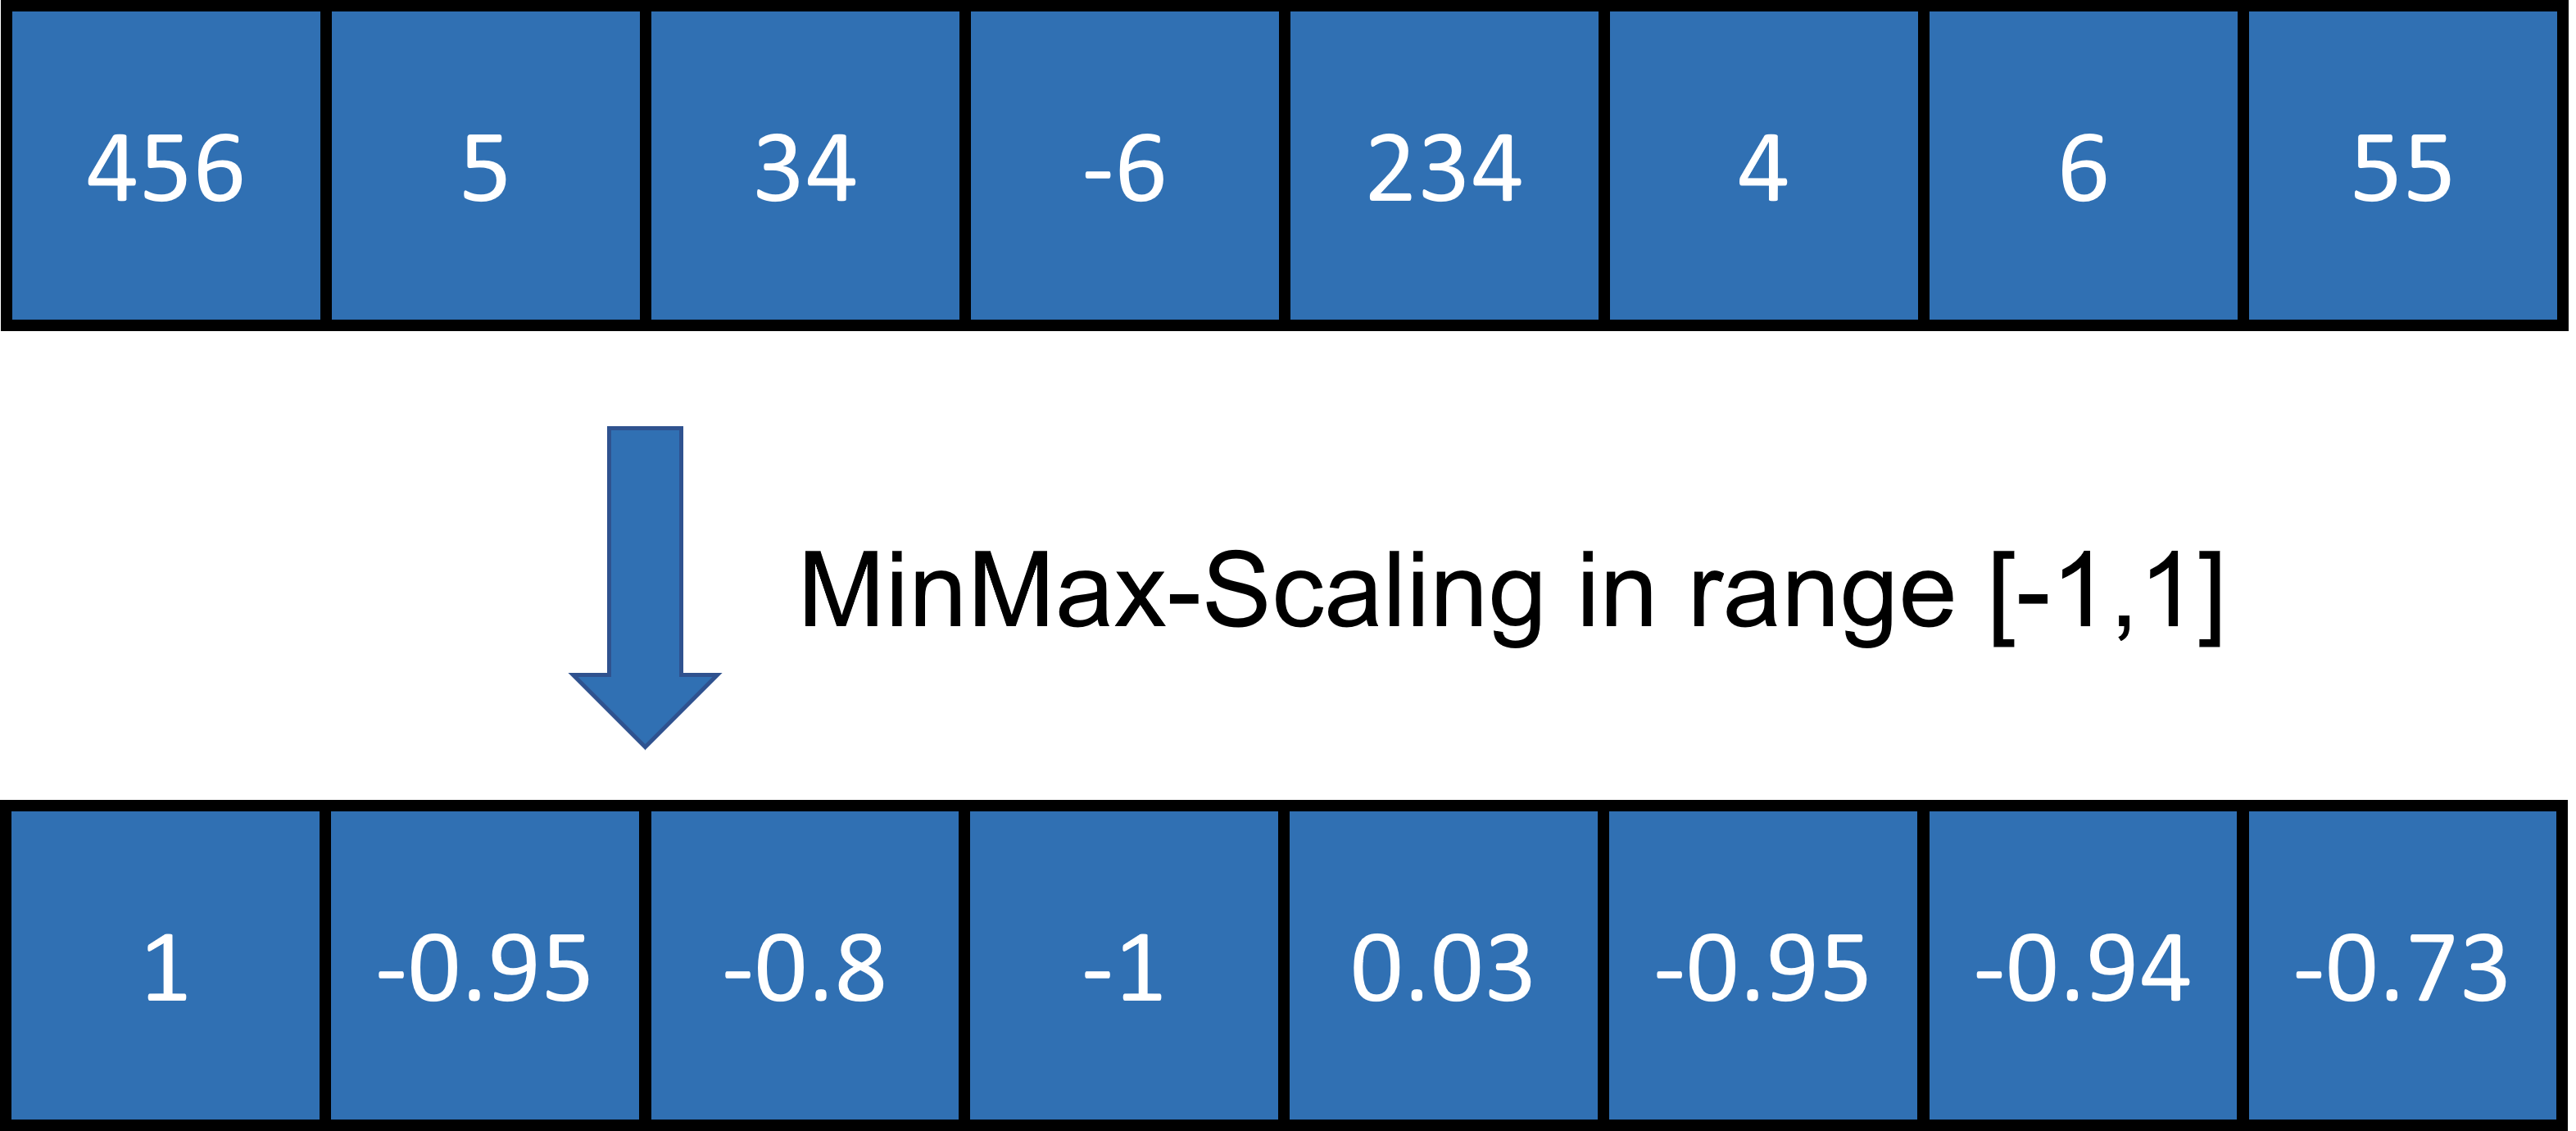
\includegraphics[width=0.5\linewidth]{IMGs/MM.png}
	\caption{Applying a MinMax-Scaler to a feature vector}
	\label{fig:MM}
\end{figure}


\subsubsection*{Hyperparameter}
Before a ML model can be trained, a set of hyperparameters needs to be defined that characterize the model and its behavior.
Most of the time, they are set manually, relying on the user's intuition or taken from literature \cite{Philipp}. 
For optimal performance, it requires extensive knowledge of the selected algorithm and how different combinations of parameters affect each other.
Exemplary hyperparameters are: learning rate, loss function, activation function or weights of neurons in NN (see chapter \ref{NN chapter}) \cite{Yang2}.
As hyperparameters play a very important role in the success of a ML model, specialized algorithms are in development for optimal hyperparameter selection \cite{Bergstra}.


\subsubsection*{K-fold Cross Validation}\label{KCV}
K-fold Cross Validation (KCV), is an approach for error estimation of ML models \cite{Zhang}. By applying KCV, the data-set is split into k subsets. All but one subset are used for training and the remaining one is used to measure the model's performance after it is trained. For that, the error-function is used. The score is saved, and the process is repeated for all k subsets \cite{Yoshua}. In the end, all k subsets were used once to assess the model. The expected value over all k-iterations is the final estimation of the models' performance. By employing this process, the model's sensitivity to one particular data-set does not influence the final rating of the model's performance \cite{Bishop}.



%https://web.archive.org/web/20170829124122id_/https://www.elen.ucl.ac.be/Proceedings/esann/esannpdf/es2012-62.pdf
%https://link.springer.com/article/10.1007/s11222-009-9153-8
%https://ieeexplore.ieee.org/abstract/document/8698831


\subsection{Core Functionalities in Machine Learning}
The core functionalities of ML are Supervised Learning, Unsupervised Learning and Reinforcement Learning (RL) \cite{Theodoridis,Janiesch}. In the following, these three functionalities are discussed in more detail.
Semisupervised Learning is a mix of Supervised and Unsupervised Learning~\cite{Zhu}. Due to its rarity and specialized approach, it is not covered by the scope of this thesis.

\subsubsection*{Supervised Learning}\label{SUPER}
Supervised Learning is split up into two parts: \textbf{Classification} and \textbf{Regression} \cite{Janiesch,Theodoridis}.

In the case of \textbf{Classification}, the data element that a model is trained on has a label (class label)~\cite{Carleo}. For example, images that contain either cats or dogs. The image is the data. The label is a corresponding value of either 1 or 0, which represents the presence of either animal in one specific image (for example, 0 for cats and 1 for dogs). The goal is to predict if a new image contains cats or dogs. The model that is used in the case of Classification is called a classifier~\cite{Theodoridis}.

To return the correct label, the classifier has to train on the available trainig-set, and find correlations between the data and labels~\cite{Carleo}.
After each training cycle, the prediction of the classifier can be compared to the true label (ground truth) and thus supervised on its performance.
\newpage
The classifier must learn the underlying structure (the pattern) of images and has to generalize, as the pictures in the test-set are not used in training and thus are unseen \cite{Bishop}. 
The found patterns allow the classification of the input (image) into discrete and limited variables (type of animal, 0 or 1) \cite{Theodoridis}.

Figure \ref{fig:CATDOG} shows a schematic representation of how a classifier is trained on a data-set containing images of either dogs or cats and how it is used to predict the label of a new image.

\begin{figure}[H]
	\centering
	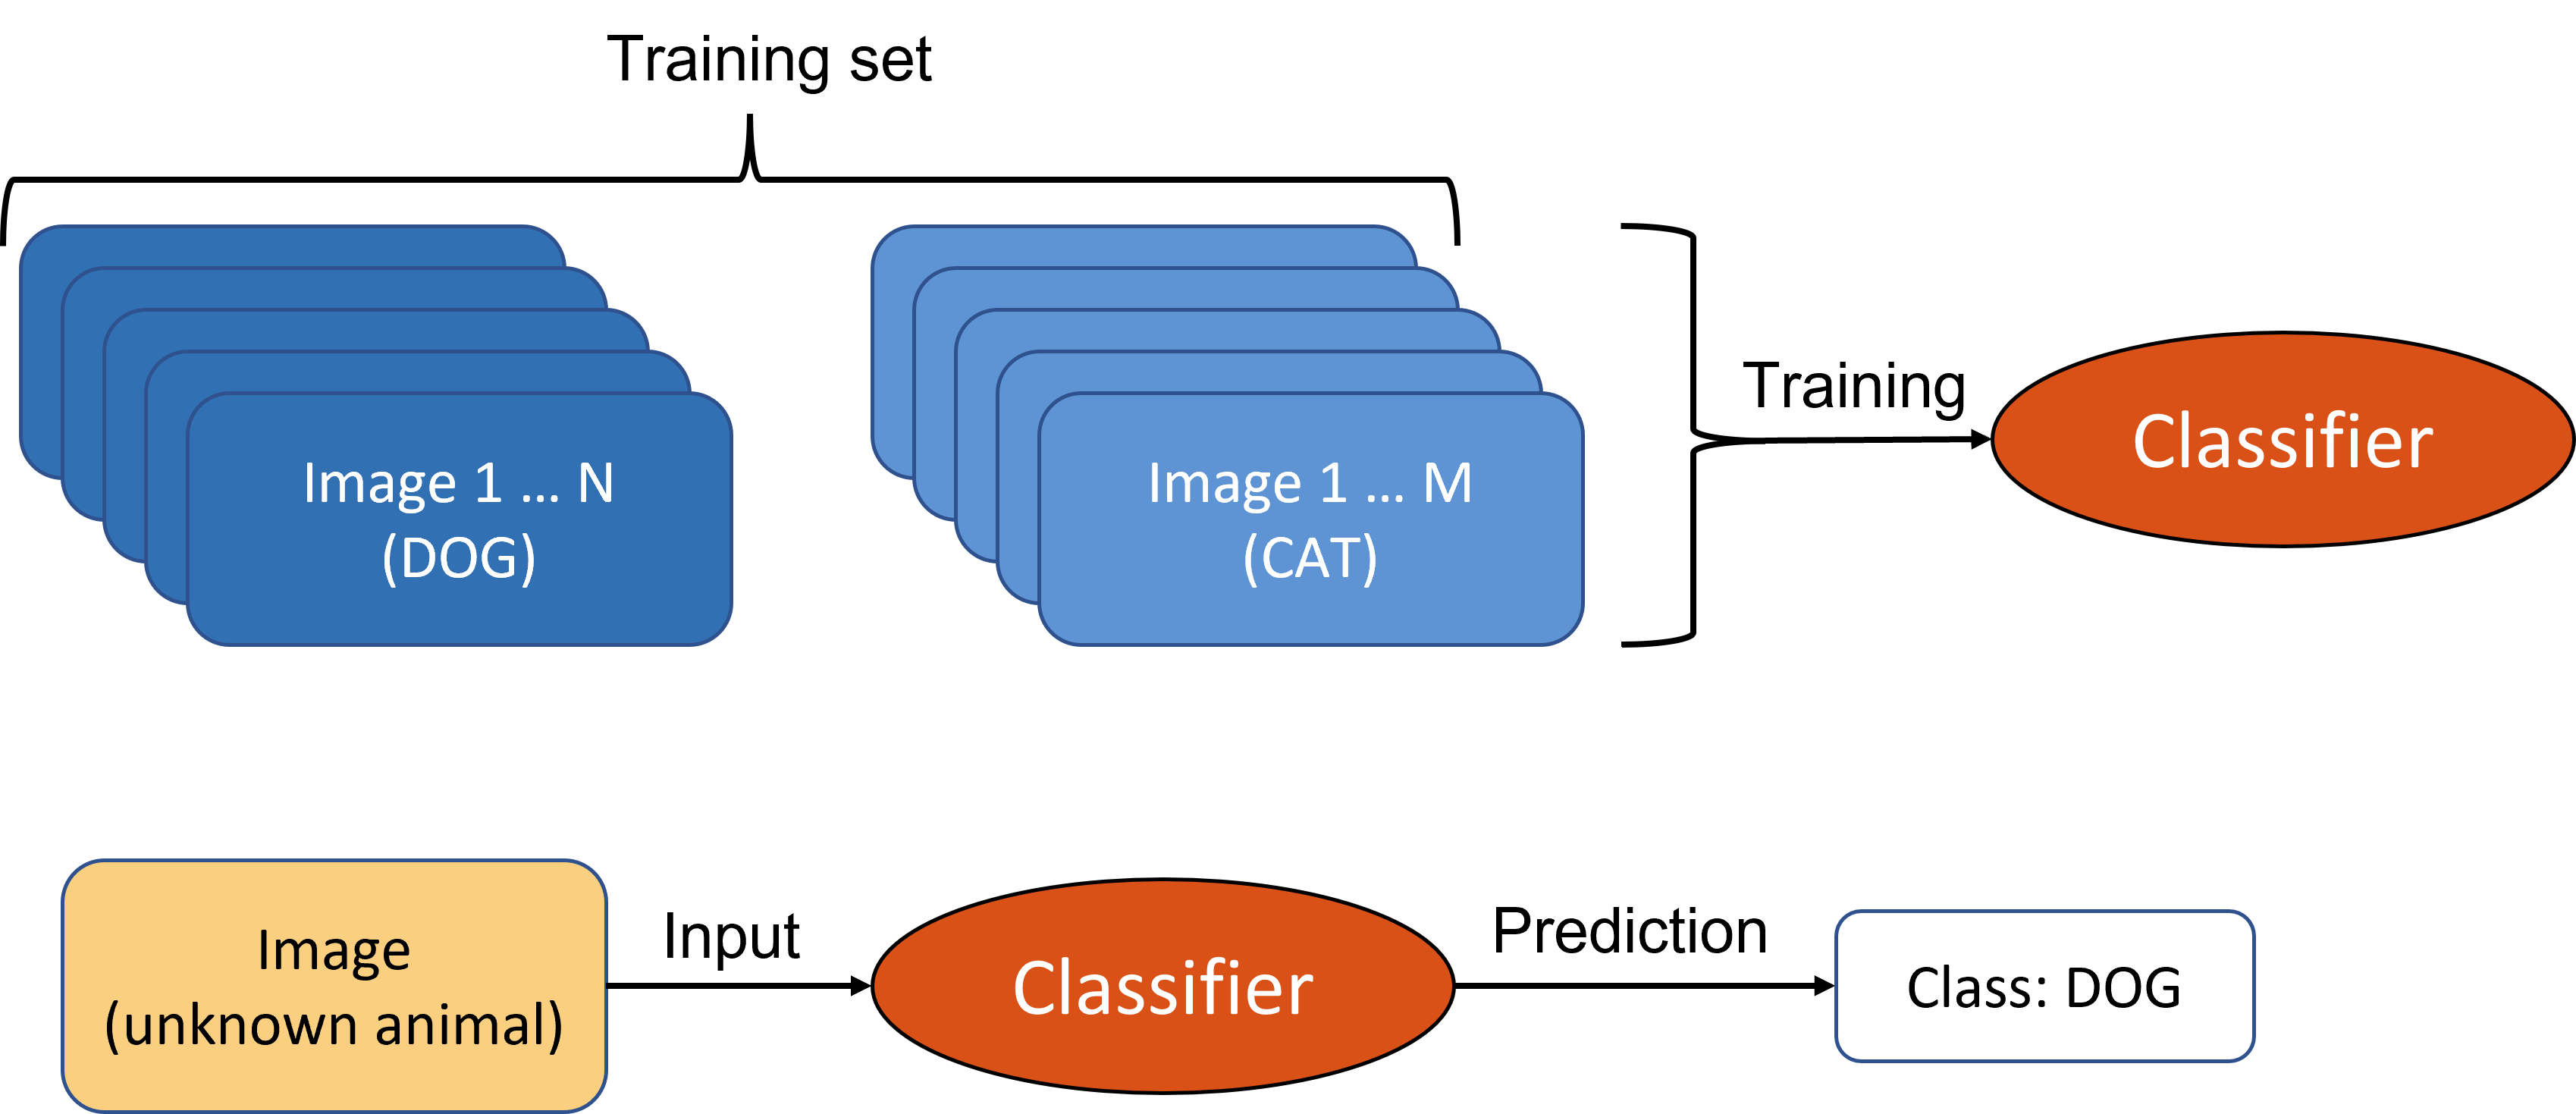
\includegraphics[width=0.9\linewidth]{IMGs/CATDOG.png}
	\caption{A schematic of the training and use of a classifier}
	\label{fig:CATDOG}
\end{figure}



Further examples of classifications are: the prediction of whether a tumor is benign or malignant or the authorship of a given text \cite{Theodoridis}.


The same basic principle is applied to \textbf{regression}. The main difference is that in the case of regression, the output is not a binary class but a continuous variable. In other words, the labels are lying in an interval. In broader terms, it is possible to call it a "curve fitting" method (see chapter \ref{TT}) \cite{Theodoridis}.

One application, for example, is to predict the position of the sun based on a picture containing shadows. The data in this case is, just as in the classification, the image. The label, on the other hand, is now a number that is the solar azimuth angle. The model can fit a function to the available data points and predict the sun's position on a new (unseen) picture.
An even more simple example is shown in figure \ref{fig:SimpleRegression}. A given data-set contains values of points in the \(x\)-\(y\) plane. With a regression model, the mapping function is estimated. Now the estimated function can be used to predict the \(y\)-value for a new \(x\)-value. 

\begin{figure}[H]
	\centering
	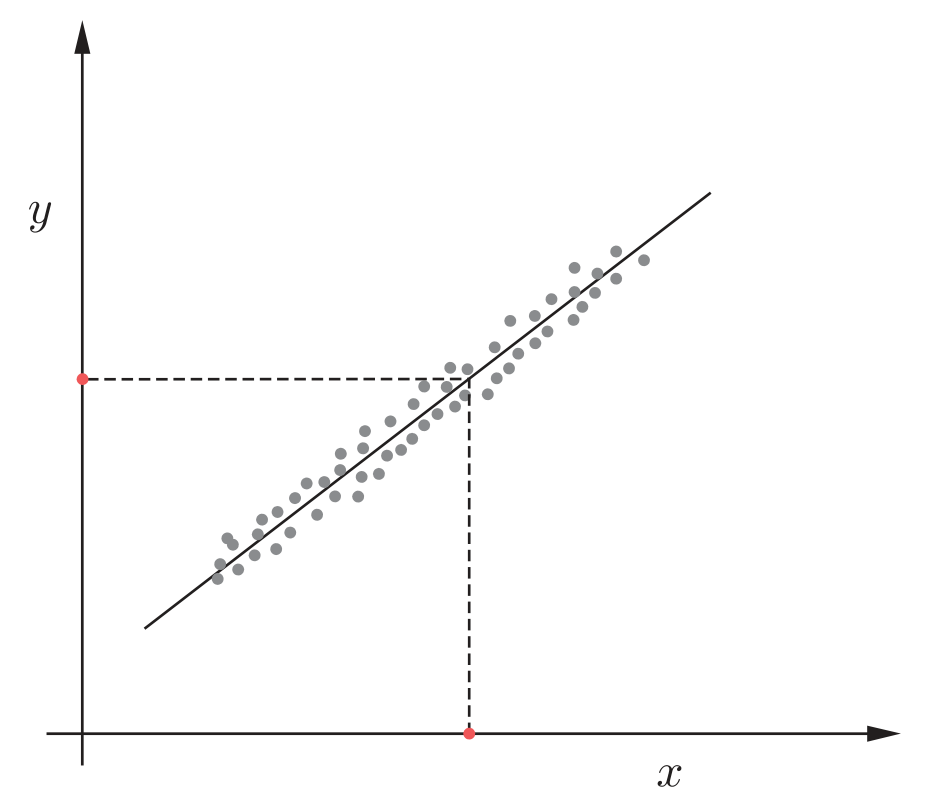
\includegraphics[width=0.5\linewidth]{IMGs/SimpleRegression.png}
	\caption{A mapping function based on a data-set containing \(x\) and \(y\) values \cite{Theodoridis}}
	\label{fig:SimpleRegression}
\end{figure}


Another example of regression is to predict a stock price in the next few minutes based on the history of the last 30 minutes \cite{Janiesch}.



\subsubsection*{Unsupervised Learning}
In Unsupervised Learning, the data that is given to a model has no labels. The goal of that method (just like in Supervised Learning) is to also find underlying patterns \cite{Carleo}. But instead of learning a pattern and comparing the output to the ground-truth, the method is designed in such a way that it discovers a pattern on its own \cite{Murphy}. The focus is not on assigning labels to an input, but on deciding to which class it belongs.

When applying this method to images, the output of the model are groups of pictures, where every group has something in common. Unsupervised Learning is very similar to human learning, as most things are learned without someone explicitly explaining how something works \cite{Murphy}. As mentioned in section \ref{Advantages and Problems of Machine Learning}, large labeled datasets are very difficult to create. Unsupervised Learning does not require a label and is thus widely applicable.

Figure \ref{fig:USL} visualizes how an unsupervised learning approach can divide a set of shapes based on their geometric properties. Class 1 contains shapes that are mostly round and class 2 contains shapes that are angular. 

\begin{figure}[H]
	\centering
	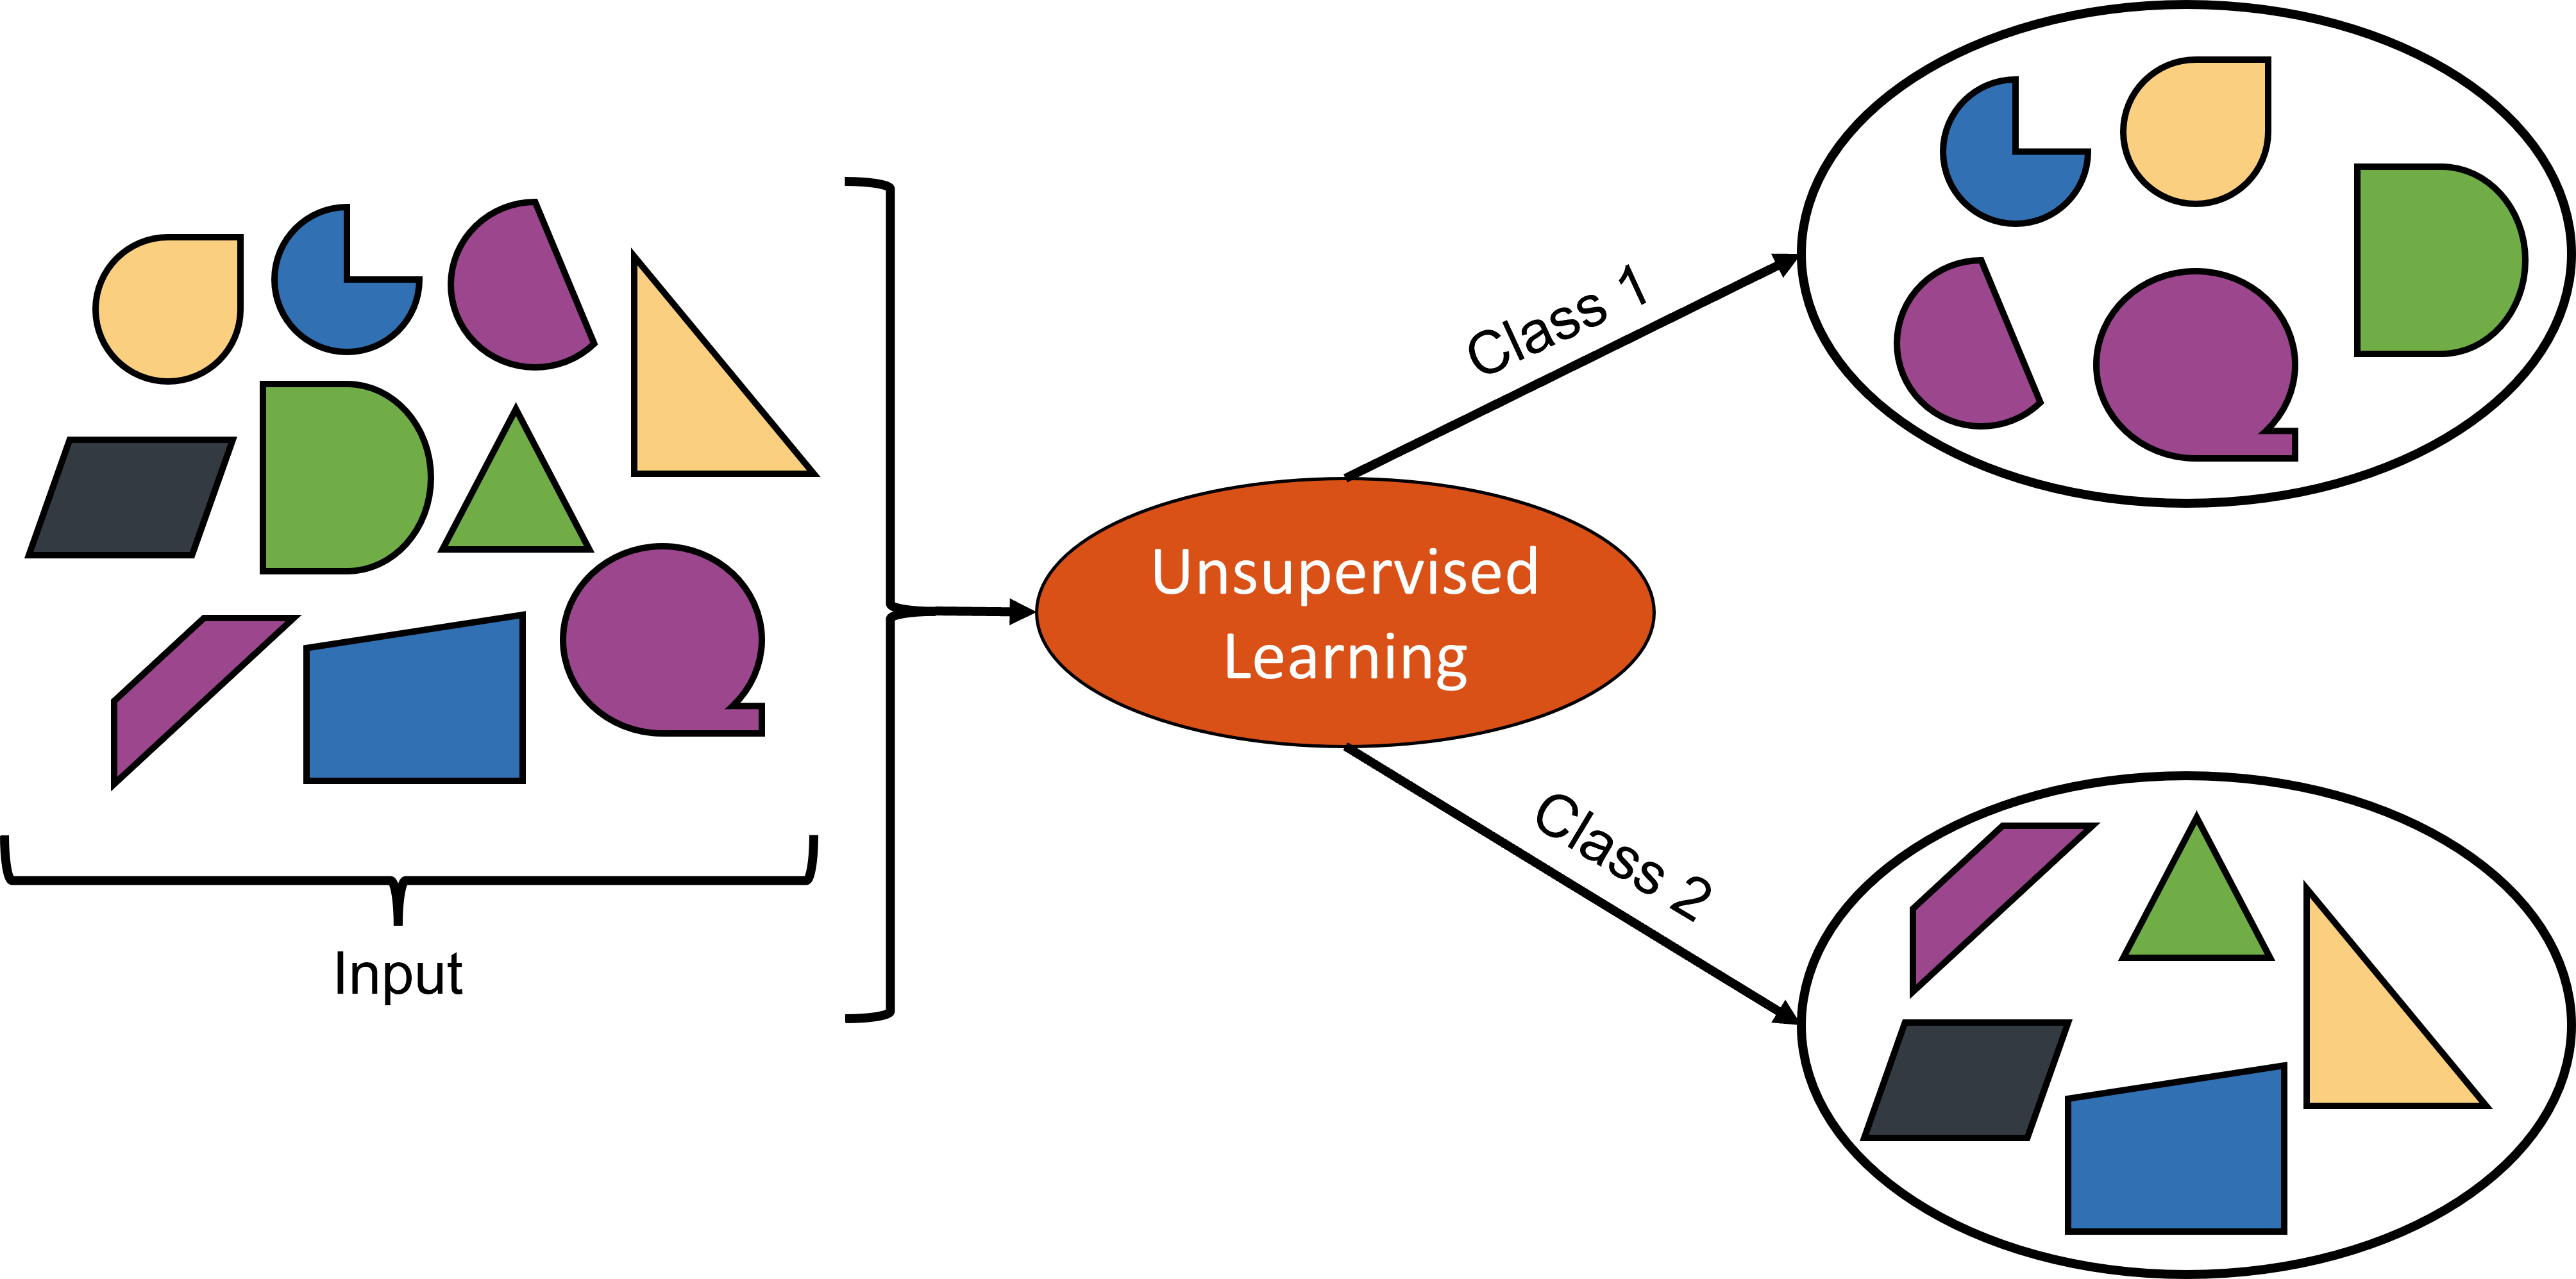
\includegraphics[width=0.9\linewidth]{IMGs/USL.png}
 	\caption{Finding similarities in shapes and grouping them into classes}
 	\label{fig:USL}
\end{figure}


\subsubsection*{Reinforcement Learning}

RL is based on the same principle as the learning process in people or animals. The main objective is to reach a goal or, in other words, to maximize a numerical value. The learning process is in a loop with observing and decision-making. The so-called agent is in an environment that he can observe and perform action in. The actions are rewarded or punished with a numerical reward. \cite{LEX}
 
Actions that bring the agent closer to the goal are rewarded proportionally to their usefulness in achieving the goal. After completion of the task (achieving the goal) a large reward is issued to signal the agent that the steps taken were successful. As the agent does not know which actions lead to high rewards, it has a significant exploration part in the beginning of its training to confirm or update its assumptions regarding the predicted reward for each action in each state.~\cite{Sutton}

One of the most challenging tasks in RL is deciding which steps in the process were the good and bad ones. This is also called the "Credit Assignment Problem" \cite{Minsky,Bishop}. To solve a task, for example, finding a way out of a labyrinth, the agent has to first navigate in the opposite direction to the exit, to then again get closer to the exit. The three distinguishing parts of RL are: a closed loop system, no clear instructions, and the long-term strategy of the agent. \cite{Sutton}

Figure \ref{fig:SimpleRL} shows one iteration of the interaction of the agent with the environment. First, the agent receives the state of the environment as a feature vector. Based on that current state and the agent's long-term strategy, it performs an action and thus changes the environment. After performing the action, the agent is rewarded for its performance based on the defined goal~\cite{LEX}.

\begin{figure}[H]
	\centering
	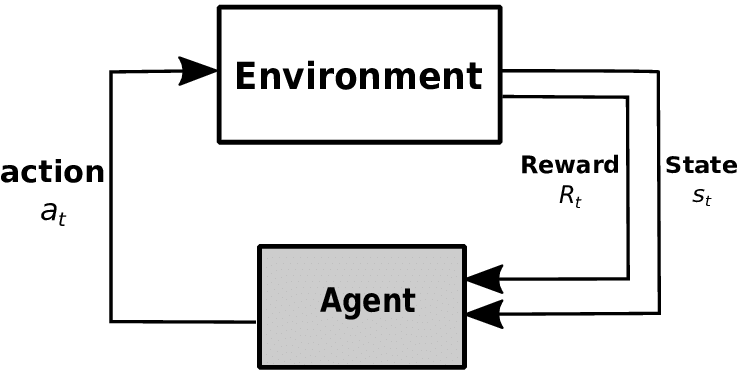
\includegraphics[width=0.5\linewidth]{IMGs/SimpleRL.png}
	\caption{The interaction of an agent with its environment in RL \cite{LEX}.}
	\label{fig:SimpleRL}
\end{figure}
RL finds a lot of applications in games and game-like scenarios, as the goal and reward are easily defined and the state of the environment is easily encoded into a feature vector \cite{Takuma}.
Due to the limited scope of this thesis and the nature of the problem described in chapter \ref{prob}, RL is not further discussed. More information can be found in \cite{Sutton}.
 

\subsection{Specialized Machine Learning Approaches}
In the following, three specialized architectures are presented and analyzed in more detail.
\subsubsection*{Neural Networks}\label{NN chapter}
NNs are based on the same principle as the functionality of the human brain \cite{Janiesch}.
The basic components of a NN in a living organism are neurons and synapses. The synapses are connecting the neurons with each other. Based on the input, a synapse can be activated or inhibited. Based on that observation, McCulloch and Pitts implemented a simple model, called a perceptron, that mimics exactly this behavior \cite{Theodoridis}.
Figure \ref{fig:2nn} shows how two neurons are connected to each other. This principle is reproduced many times to create a large NN out of perceptrons.
\begin{figure}[H]
	\centering
	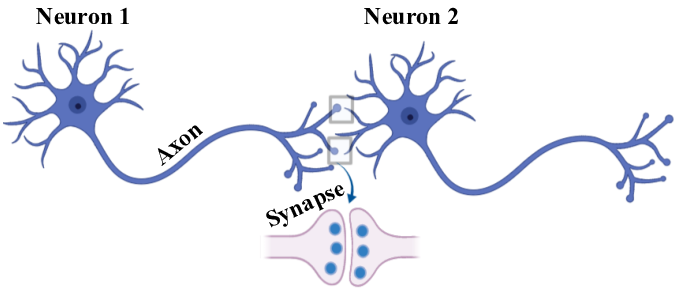
\includegraphics[width=0.8\linewidth]{IMGs/2NN.png}
	\caption{Connection of two neurons via synapses \cite{Das}}
	\label{fig:2nn}
\end{figure}
\newpage
NN are also referred to as Artificial Neural Networks (ANNs). These models are based on the same principle as the perceptron. In this case, the perceptrons are arranged in layers and referred to as nodes or neurons. The first layer is called an input layer and the last one is the output layer. The layers in between are called hidden layers \cite{JOOST}. 

Figure \ref{fig:NN1} shows an exemplary NN with three hidden layers. Each element of the input vector is given to one node at the input layer. This type of NN is also called a Feed-Forward Neural Network. Because the neurons are fully connected, it is also referred to as a fully connected NN \cite{Sainath}. Note that the output does not need to be a single value. It can also be a vector. In that case, the output layer would consist of multiple nodes.

\begin{figure}[H]
	\centering
	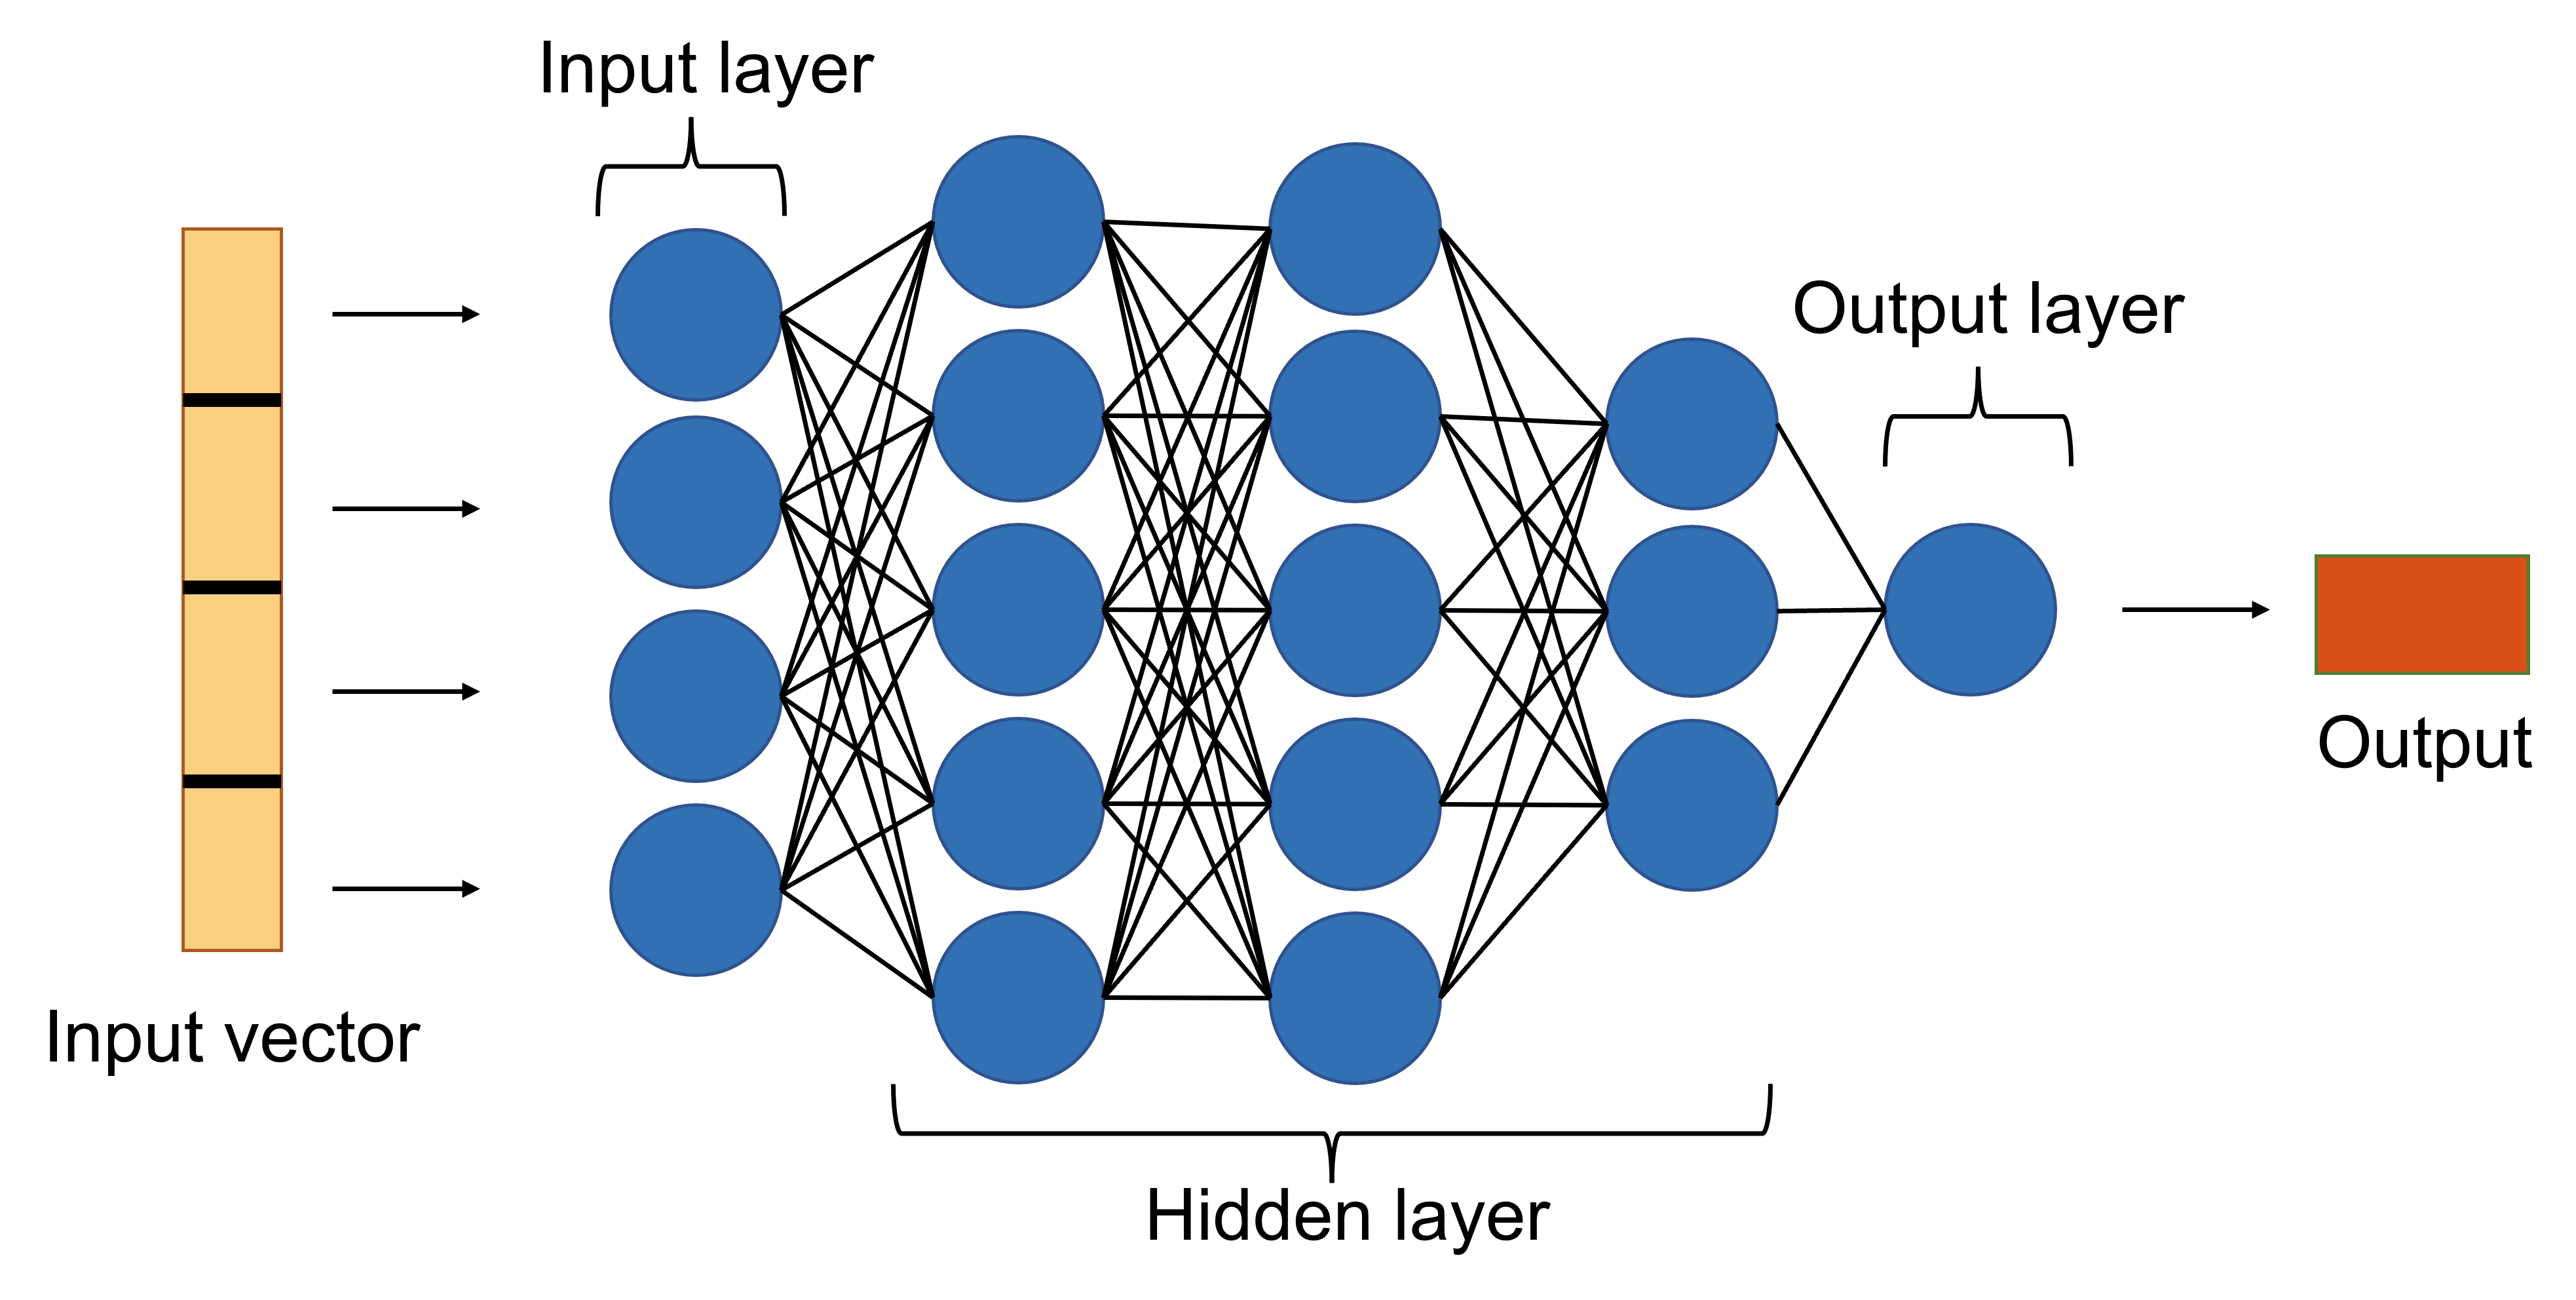
\includegraphics[width=0.8\linewidth]{IMGs/NN1.png}
	\caption{NN with three hidden layers}
	\label{fig:NN1}
\end{figure}
 
To model an organic NN more closely and improve the performance, the nodes have an activation function built into them, which can introduce non-linearity \cite{Goyal}. One of the most common activation functions is the "rectified linear unit" (ReLU) \cite{Goodfellow}. Figure \ref{fig:AF} shows three common activation functions. The most common activation functions are: ReLU, sigmoid, tanh and softmax \cite{Activation}

\begin{figure}[H]
	\centering
	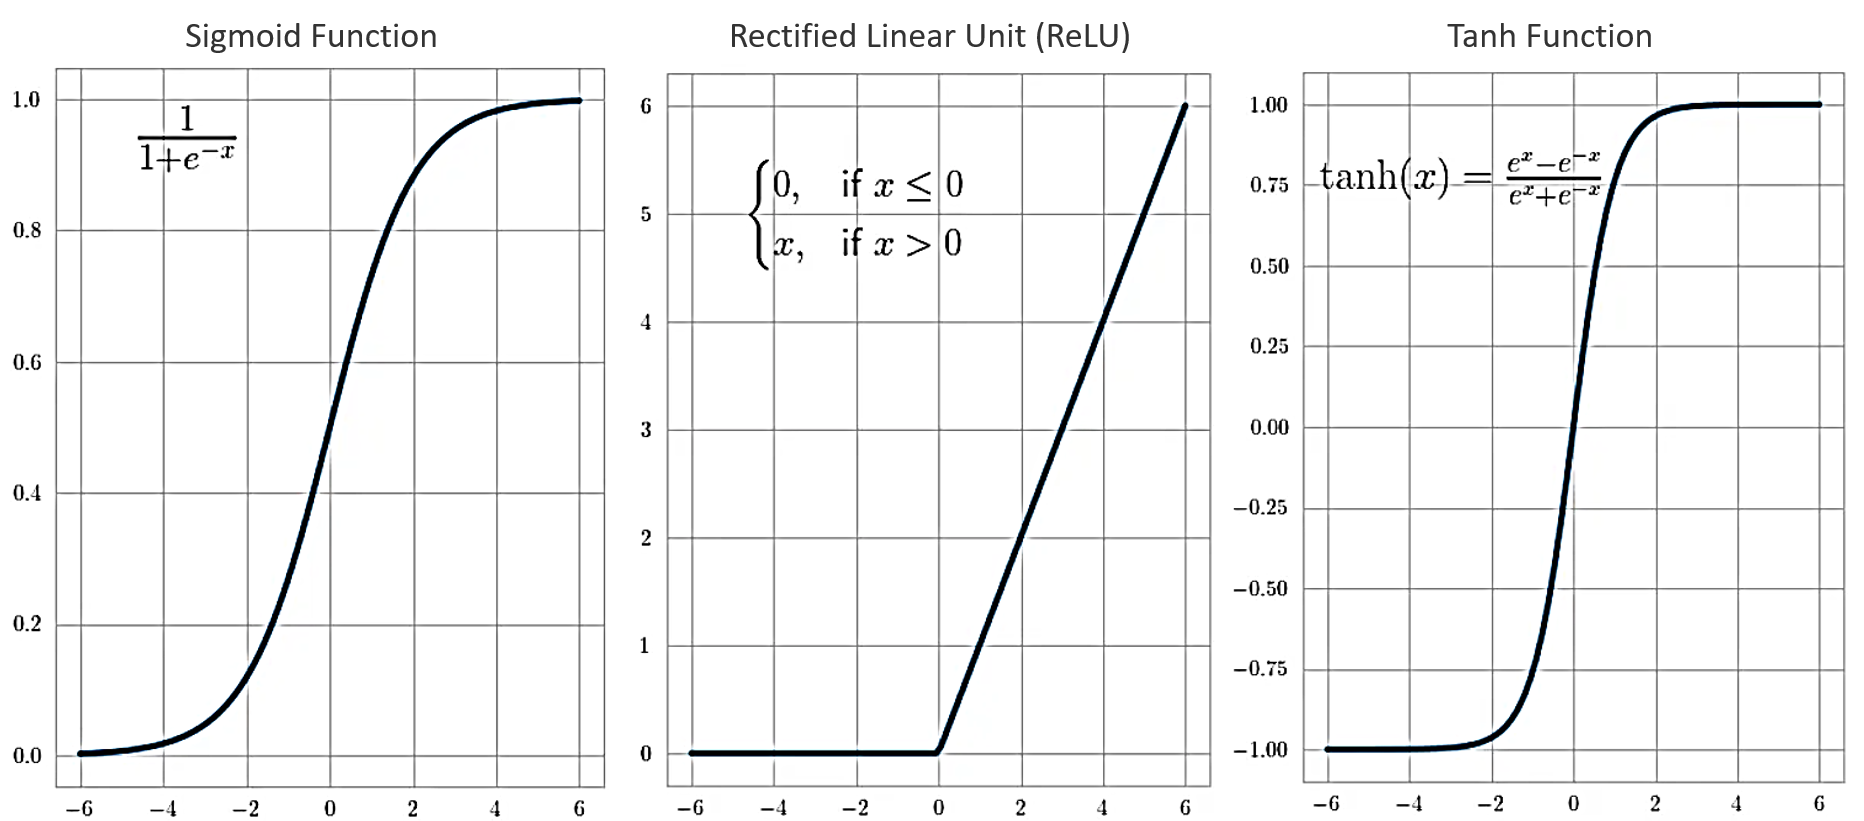
\includegraphics[width=0.8\linewidth]{IMGs/Active.png}
	\caption{Various activation functions for NNs \cite{Activation}}
	\label{fig:AF}
\end{figure}

Figure \ref{fig:PC} shows the basic functionality of a neuron at the first hidden layer. The ouput-elements of the input layer are pre-multiplied with individual values called weights and summed up to a single value. This value is processed by the activation function and returns the output for that specific neuron for that specific input \cite{BattaMahesh}. The output value is then used as input in the following hidden layers \cite{Ding}. The adjustments of those weights is done in training through a process called back-propagation \cite{Chauvin}. 
It is important to note that the activation functions can be chosen for each layer individually. Especially in classification, the activation function at the output layer is most commonly set as SoftMax while in the previous layers as ReLU \cite{Asadi}. 

\begin{figure}[H]
	\centering
	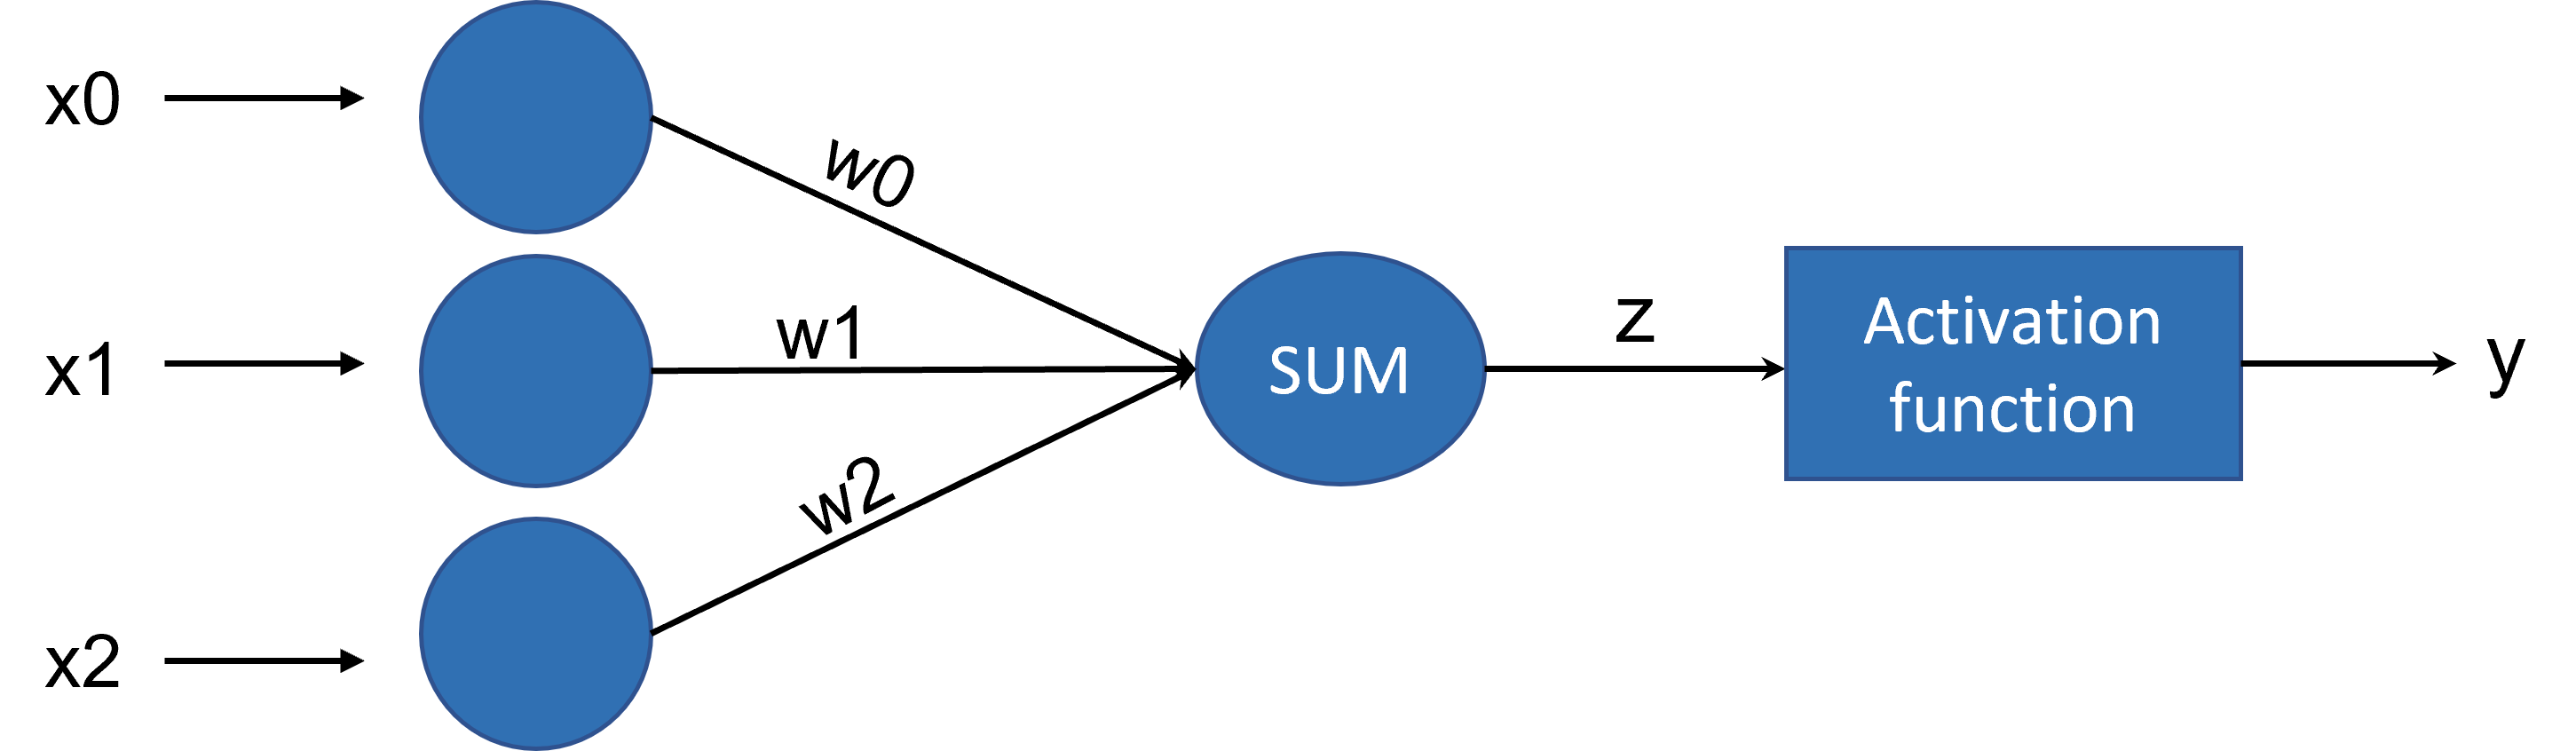
\includegraphics[width=0.8\linewidth]{IMGs/PEC.png}
	\caption{Graphical representation of a perceptron \cite{Ding}}
	\label{fig:PC}
\end{figure}

Deep Neural Networks (DNNs) are NNs that contain many hidden layers. The increased amount of parameters and non-linearity helps them achieve better feature abstraction and learn more complex patterns \cite{JOOST}.
The biggest disadvantage of DNNs and DL in general is that even more data is necessary to optimally tune the free parameters \cite{Thompson}. Further, DL is very computationally expensive and requires significantly more time for training \cite{Fu}. 





\subsubsection*{Recurrent Neural Networks}
Recurrent Neural Networks (RNNs) are specialized NNs that are designed to be applied to problems involving time-series data, like sensor data or ordered data like sentences \cite{Jain}. After each input, the neurons in a RNN are sending feedback signals to the following and some previous nodes. By doing that, a cycle is formed \cite{Grossberg}. By having this feedback loop to previous nodes, the output is dependent on the new input and the output from the previous input. This specialized architecture can pay attention to the sequence of the input data \cite{Jain}.

The rest of the functionality is almost the same as in a conventional NN. Figure \ref{fig:rnn} shows a simple RNN. The output of the first layer is sent back to the nodes C1 and C2. In this case, they are called context units. With this structure, the RNN can "remember" the input from the previous input. These closed-loop cycles are the "memory" of the RNN \cite{Salehinejad}.

\begin{figure}[H]
	\centering
	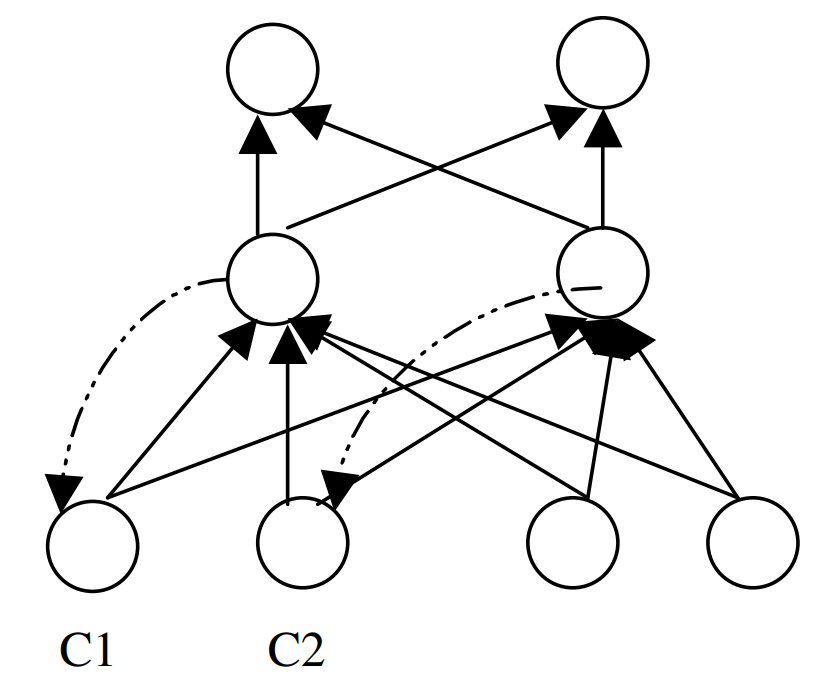
\includegraphics[width=0.4\linewidth]{IMGs/rnn.png}
	\caption{Simple RNN \cite{Jain}}
	\label{fig:rnn}
\end{figure}

By using the memory-structure, RNNs are capable of understanding sequential dependencies. A conventional RNN is capable of remembering up to ten time-steps (inputs) back. By adding more recurrent connections with the goal of increasing the memory-capacity, the gradient of the response is either exponentially increasing to infinity or decreasing to 0 \cite{Staudemeyer}. Thus, a standard RNN is limited in its ability to remember a lot of data.

Figure \ref{fig:rnn2} shows how a RNN can be unfolded. The recurrent structure is unfolded in the time-domain and gives a clear understanding of how the output of a cell at time \(t_0\) is used as additional input at time \(t_1\).

\begin{figure}[H]
	\centering
	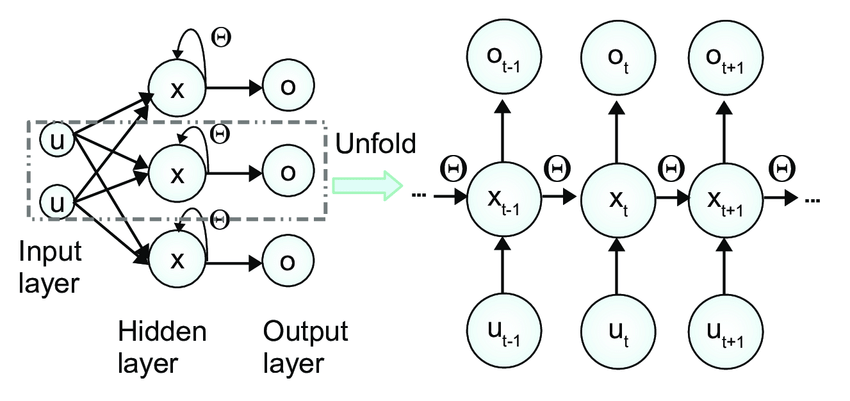
\includegraphics[width=0.8\linewidth]{IMGs/RNN2.png}
	\caption{Unfolded structure of a RNN \cite{Guo}.}
	\label{fig:rnn2}
\end{figure}


A subgroup of RNNs are long-short- term memory RNNs (LSTMs). LSTMs are able to learn correlation of even longer sequences than conventional RNNs \cite{Salehinejad}. LSTMs are capable of remembering more than 1,000 time-steps \cite{Staudemeyer}.

LSTM-networks are finding more and more areas of application. For example, in machine health monitoring or load prediction in power stations \cite{Zhao,Muzaffar}. The similarity between those applications is the dependency of the output on recent and past inputs. 

\subsubsection*{Physics Informed Neural Networks}
Physics-informed Neural Networks (PINNs) are special types of NNs that are capable of following defined boundary conditions like laws of physics \cite{Cai}. One of the most used application domain, are problems involving partial differential equations (PDEs). Instead of using the available data to discover the physics from scratch, prior knowledge can be incorporated through the PDEs \cite{Cuomo}. By utilizing PINNs, a simple NN architecture can be used, that requires less training time, and can achieve equivalent results to large NNs \cite{Misyris}.

Figure \ref{fig:piml} shows the basic functionality of a PINN. The overall goal is to minimize the error function, just as in function fitting (see chapter \ref{TT}). In this case, the error function is made up of the initial- and boundary-conditions as well as the constraints of the PDE \cite{Guo}. The training process is analogue to the standard NN approach. 
\begin{figure}[H]
	\centering
	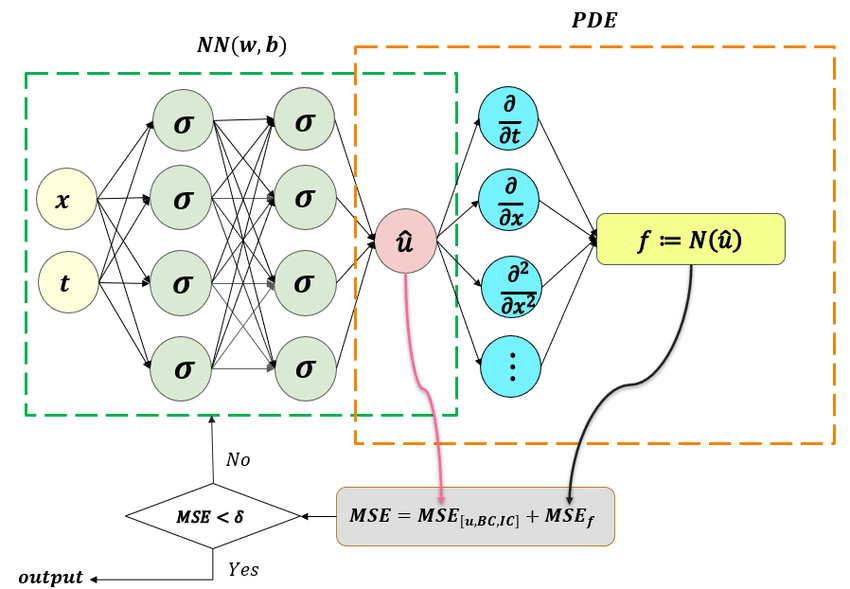
\includegraphics[width=0.7\linewidth]{IMGs/piml.png}
	\caption{Schematic diagram of a PINN \cite{Guo}.}
	\label{fig:piml}
\end{figure}




\newpage
\section{Overview of Machine Learning in Industry Applications}
In the following, the application of ML in engineering and industrial applications is discussed.
\subsection{General Application of Machine Learning in Industry}
The possibilities of ML are extending to many areas of application \cite{Deiana}. The analysis of recent publications in \cite{Bertolini}, concluded four main categories of ML for industrial applications. Table \ref{MLIND} gives to each category an example.

\begin{table}
	\begin{center}
		\begin{tabular}{|| l | l ||}
			\hline
			\rule{0pt}{2ex}Application Domain: & Example:\\
			\hline
			\hline
			\rule{0pt}{2ex}Maintenance Management & Failure modes classification and prediction\\\hline
			Quality Management & Defects detection and classification\\	\hline
			Production Planning and Control & Job scheduling and dispatching\\\hline
			Supply Chain Management & Demand planning and forecasting\\
			\hline
		\end{tabular}
		\caption{Main categories of ML for industrial applications \cite{Bertolini}.}
		\label{MLIND}
	\end{center}
	\vspace{-4mm}
\end{table}
When comparing the implemented ML-approaches, Supervised Learning clearly dominates each category. When looking at the total field, each ML-approach (Supervised, Unsupervised and RL) experienced a significant growth increase over the last 20 years \cite{Bertolini}. This is an indicating factor that ML will play an important role in the future for engineering sciences.

Condition Monitoring and Predictive Maintenance (which are both in the domain "Maintenance Management") are closely related to the explained problem in chapter \ref{prob}.
Condition monitoring is the continuous analysis of parameters that correlate to the machines operation and maintenance \cite{Rao}. Predictive Maintenance is a preventive maintenance program. Instead of scheduling maintenance activities after a failure has occurred, predictive maintenance uses condition monitoring to run the machines as long as possible (close to failure) to eliminate unnecessary downtime through premature stopping or unexpected delays through unforeseen failures \cite{Mobley}.

It is important to note that Predictive Maintenance and Condition Monitoring are also performed with other tools, like statistical analysis and do not solely rely on ML \cite{Carvalho, Divya}. 


 
\subsection{Comparison of Machine Learning in Gear Applications}
The process of calculating heath indicators has gained a lot of interest in engineering in the past years. By correctly assessing a systems' state, accidents and unexpected downtime can be avoided \cite{Wang}. In this section, the application of ML in Condition Monitoring and Predictive Maintenance of gears is analyzed.

The basis of heath indicators are signals or values coming from the physical system itself. Vibration, noise, electrical current and thermal images can be used for fault detection or to determine the state-of-damage in gears \cite{Prav,KaraACUSTIC,Medina,Kara}

By using the vibration signal, it is possible to determine gear damage like tooth cracks and face wear. These kinds of damage can introduce vibrations, that travel to other parts of the system like the gearbox housing. By having an accelerometer on the housing, the vibrations can be detected and analyzed. The proposed method in \cite{Prav} was able to successfully make a distinction between a faulty and a healthy gear. This method however, did not make any prediction regarding the progressing state of health of the gears and only analyzed them in their current state-of-damage. 

The approach in \cite{Medina} uses a LSTM network to determine the progressing level of pitting. The input signal is classified into nine levels of severity of damage. The pitting damage was created artificially by Electrical Discharging Machining (EDM). The input data is an acoustic recording of 15 seconds. In total 1215 samples are recorded. After prepossessing and encoding, the LSTM could successfully classify each signal into the correct class of pitting damage.

The method applied in \cite{RTiwari} also uses vibration signals to perform a classification. In this approach, a Support Vector Machine (SMV) is used to classify healthy and worn gears. The goal is to classified different gears based on their damage. Some gears had chipped or missing teeth. This approach also achieved a high success rate. No attention is given in regards of the change of variation over a long period of time to determine a state-of-damage. 


These approaches are not transferable to the problem described in chapter \ref{prob}. When the datasets for those methods are constructed, the gears were already in the state that is used as a label (healthy, damaged).

When trying to transfer this approach to get a better prediction than the Miner rule, the input would be the load-history and the label the true state-of-damage or range of it. But calculating the physically accurate damage sum D is not possible. Thus, these approaches are not capable of solving the problem at hand. 

Over the last decade, significant advancements are also continuously made in the area of predicting the Remaining-Useful-Life (RUL) of machine elements \cite{Deutsch,He,Yan}.
The biggest problem with those models and approaches, is the assumed constant load that is acting on the components. Due to this assumption, these approaches can not be transferred to machinery where the cyclic loads have a significant variance in amplitude over time.

In summery, no methods were published that use a-priori knowledge of the Miner rule and the known load sequence to determine a more confident state-of-damage in machine elements.

